\section{Intermediate $\AR$s with $3 < \AR < 4.75$}

We now move to the horizontal $n=1$ branch dominates by the LE vortex shedding (see figure \ref{}), i.e. to $3 \le \AR \le 4.75$, and use $\AR=4$ and $\AR=4.5$ as representative cases.

\subsection{A $2D$ bifurcation}

\subsubsection{Non linear simulations}

\begin{figure}
  \centering
  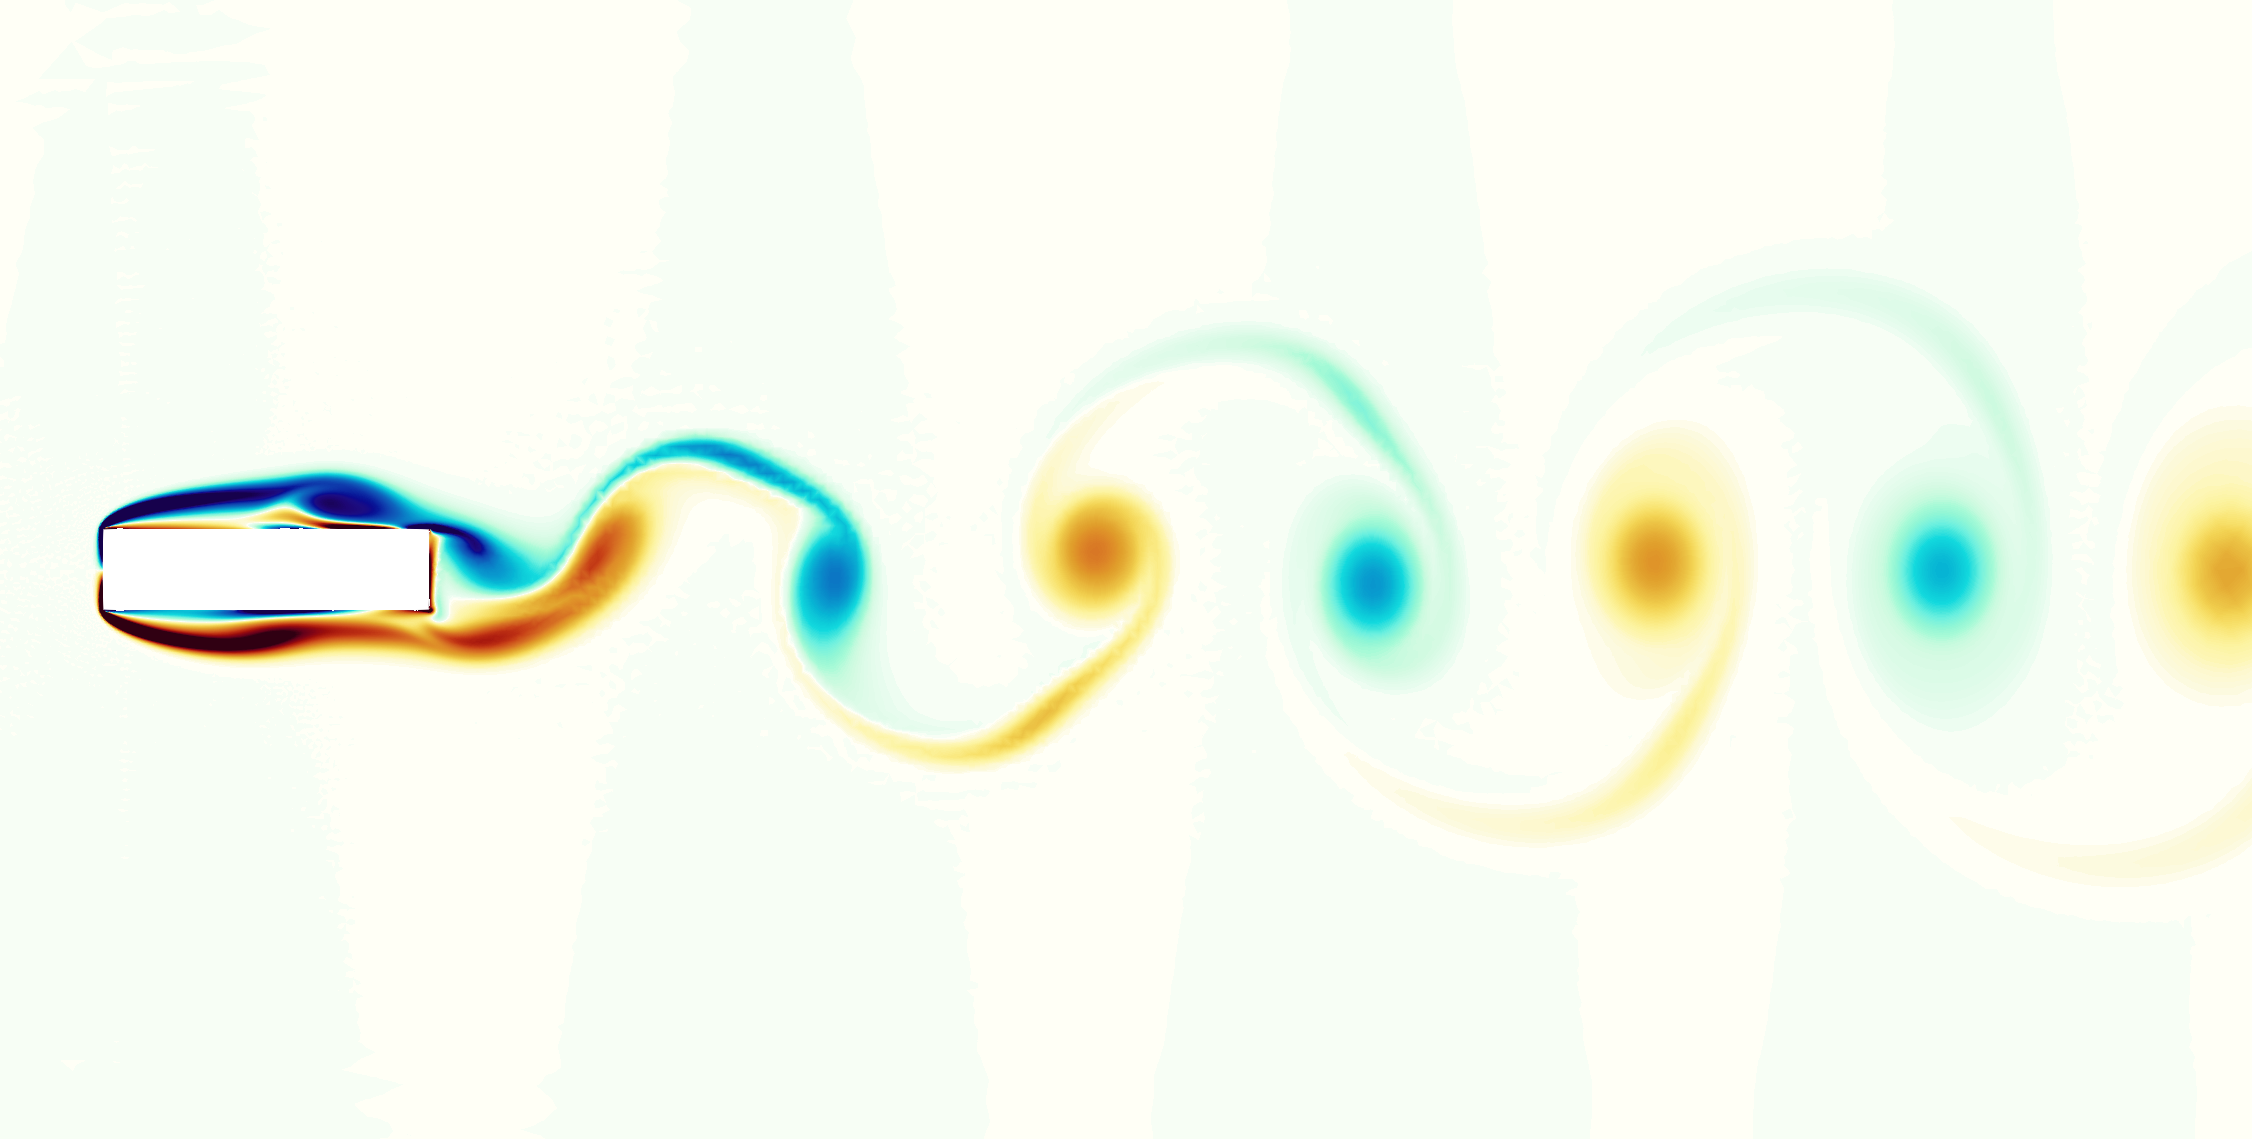
\includegraphics[trim={0 100 0 100},clip,width=0.49\textwidth]{./fig/vort_Re425_25.png}
  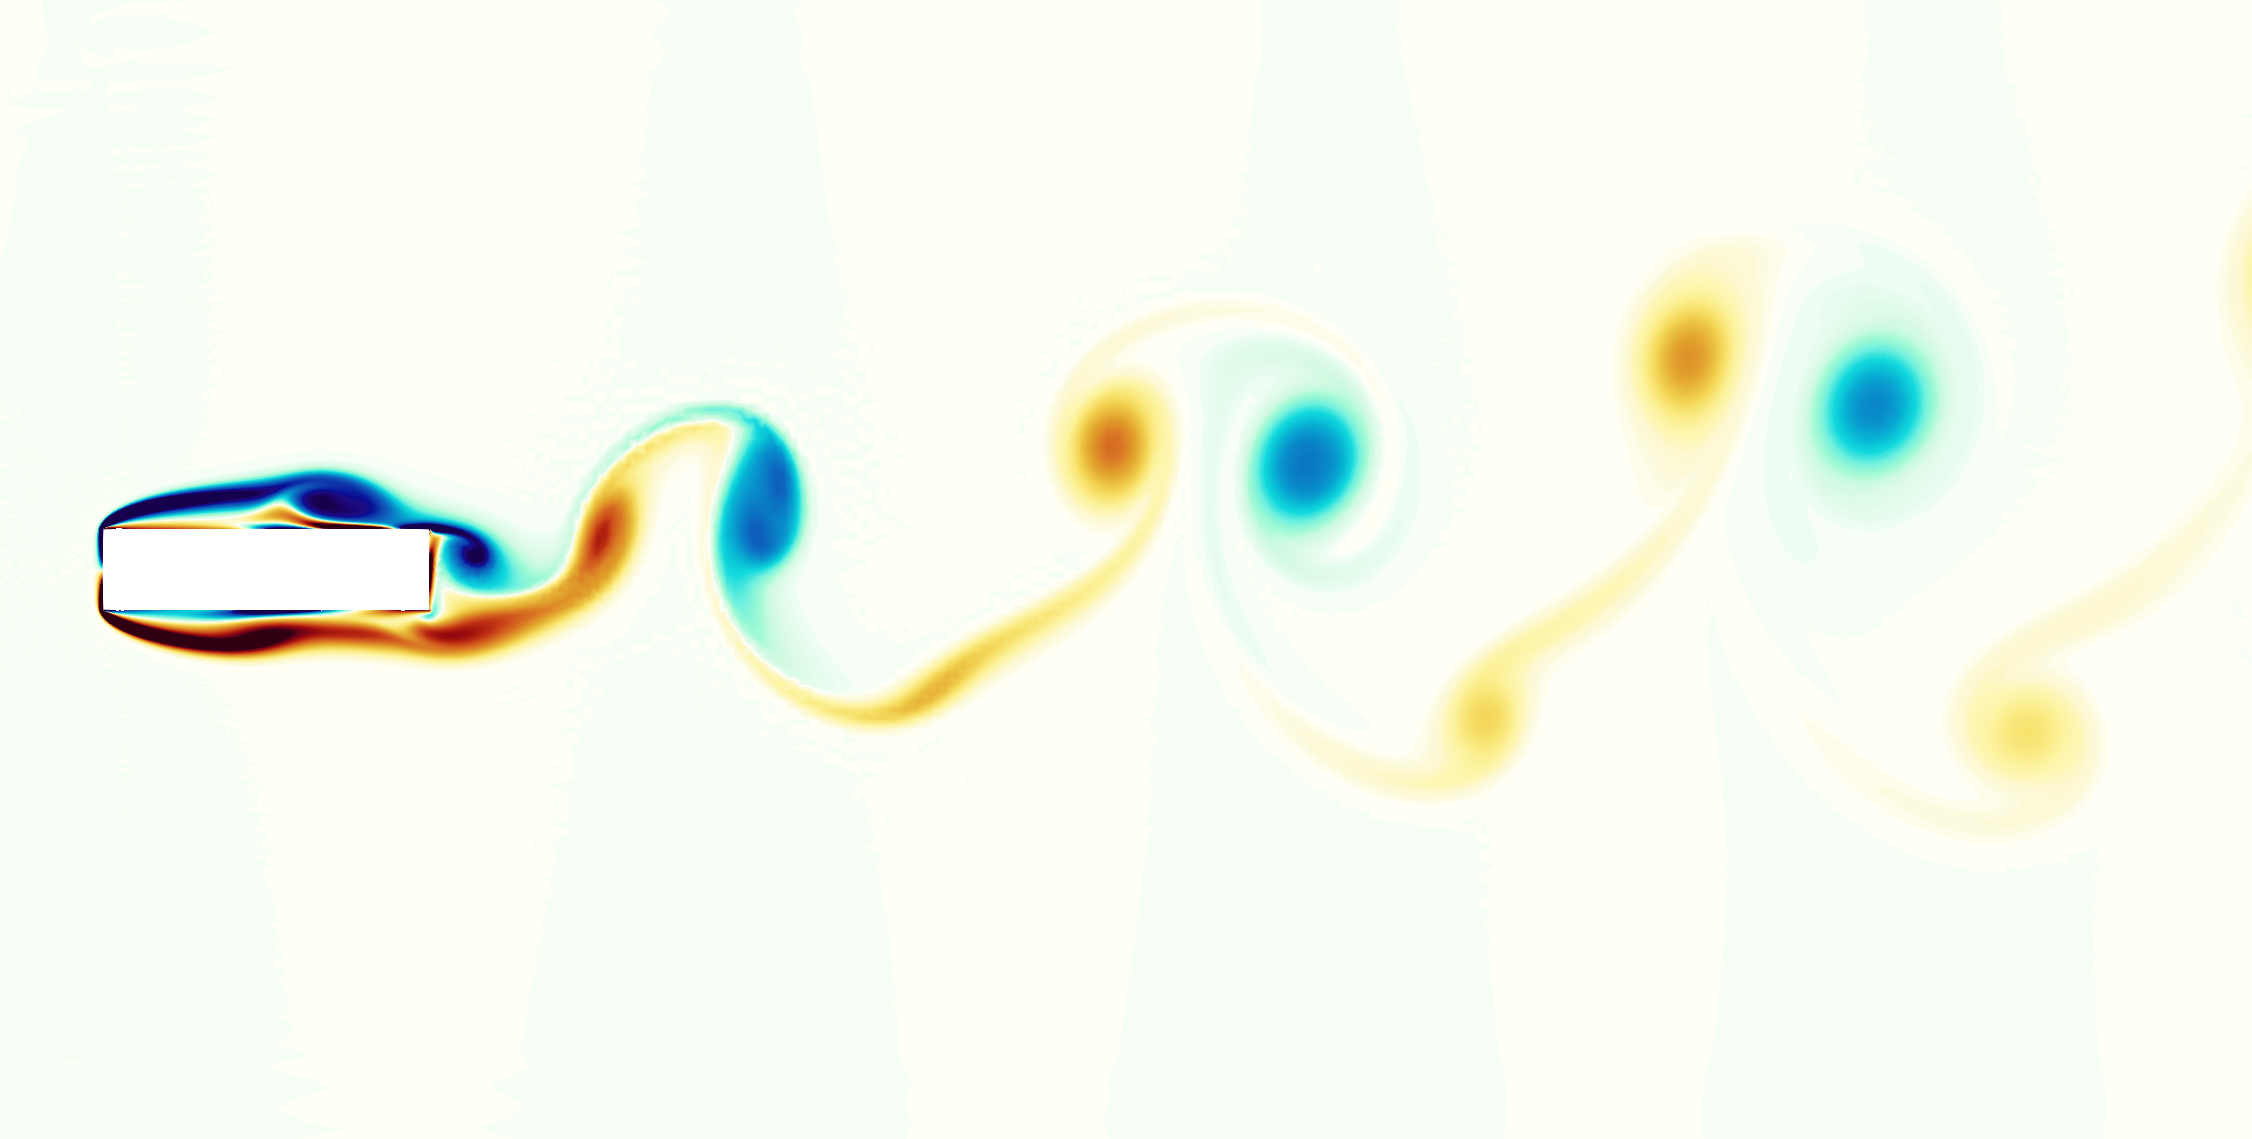
\includegraphics[trim={0 100 0 100},clip,width=0.49\textwidth]{./fig/vort_Re450_25.png}  
  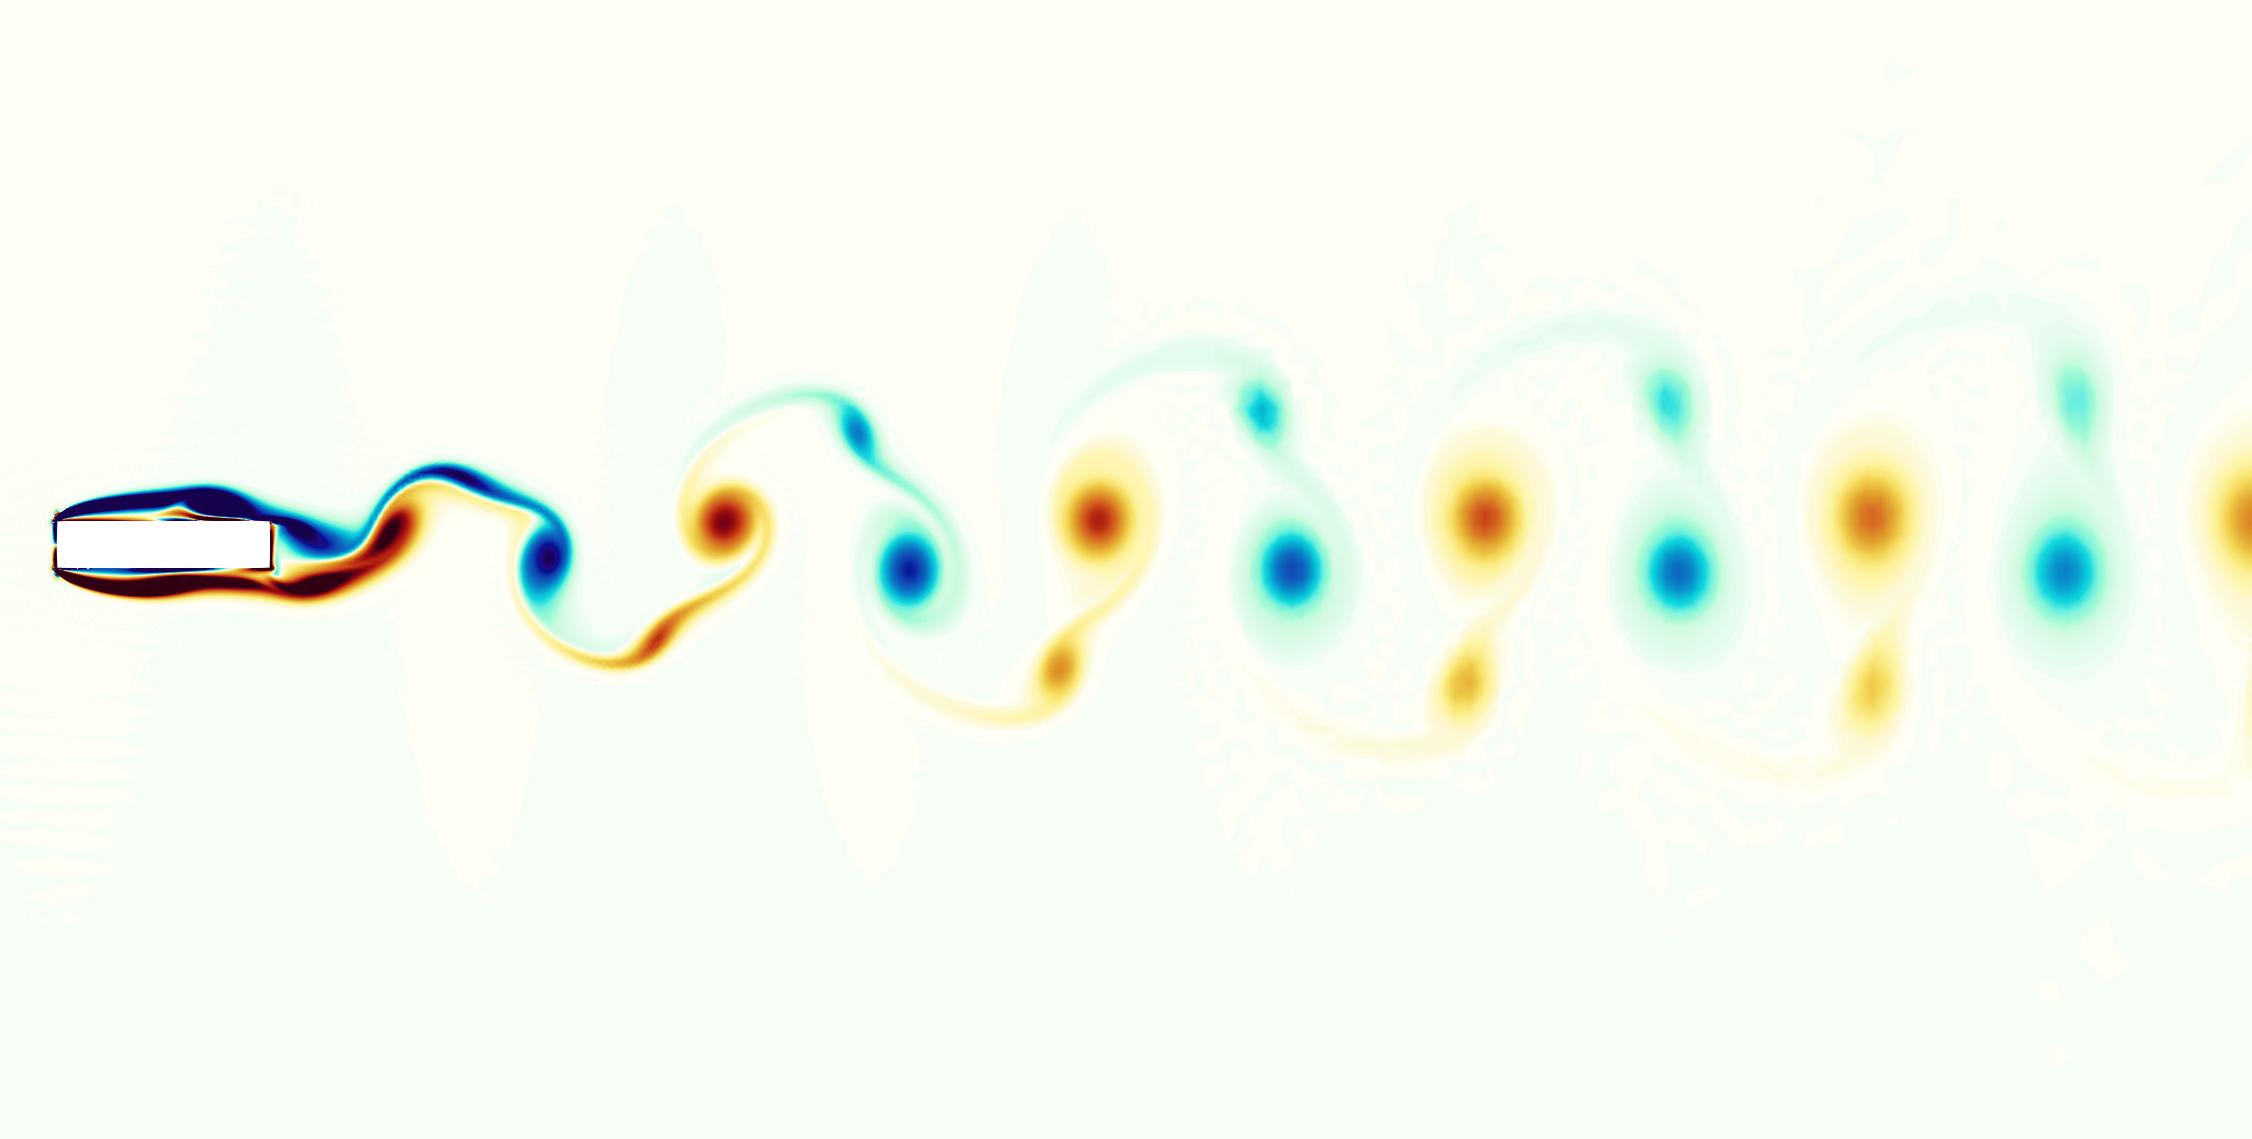
\includegraphics[trim={0 100 0 100},clip,width=0.49\textwidth]{./fig/AR4p5/vort_Re430_25.png}
  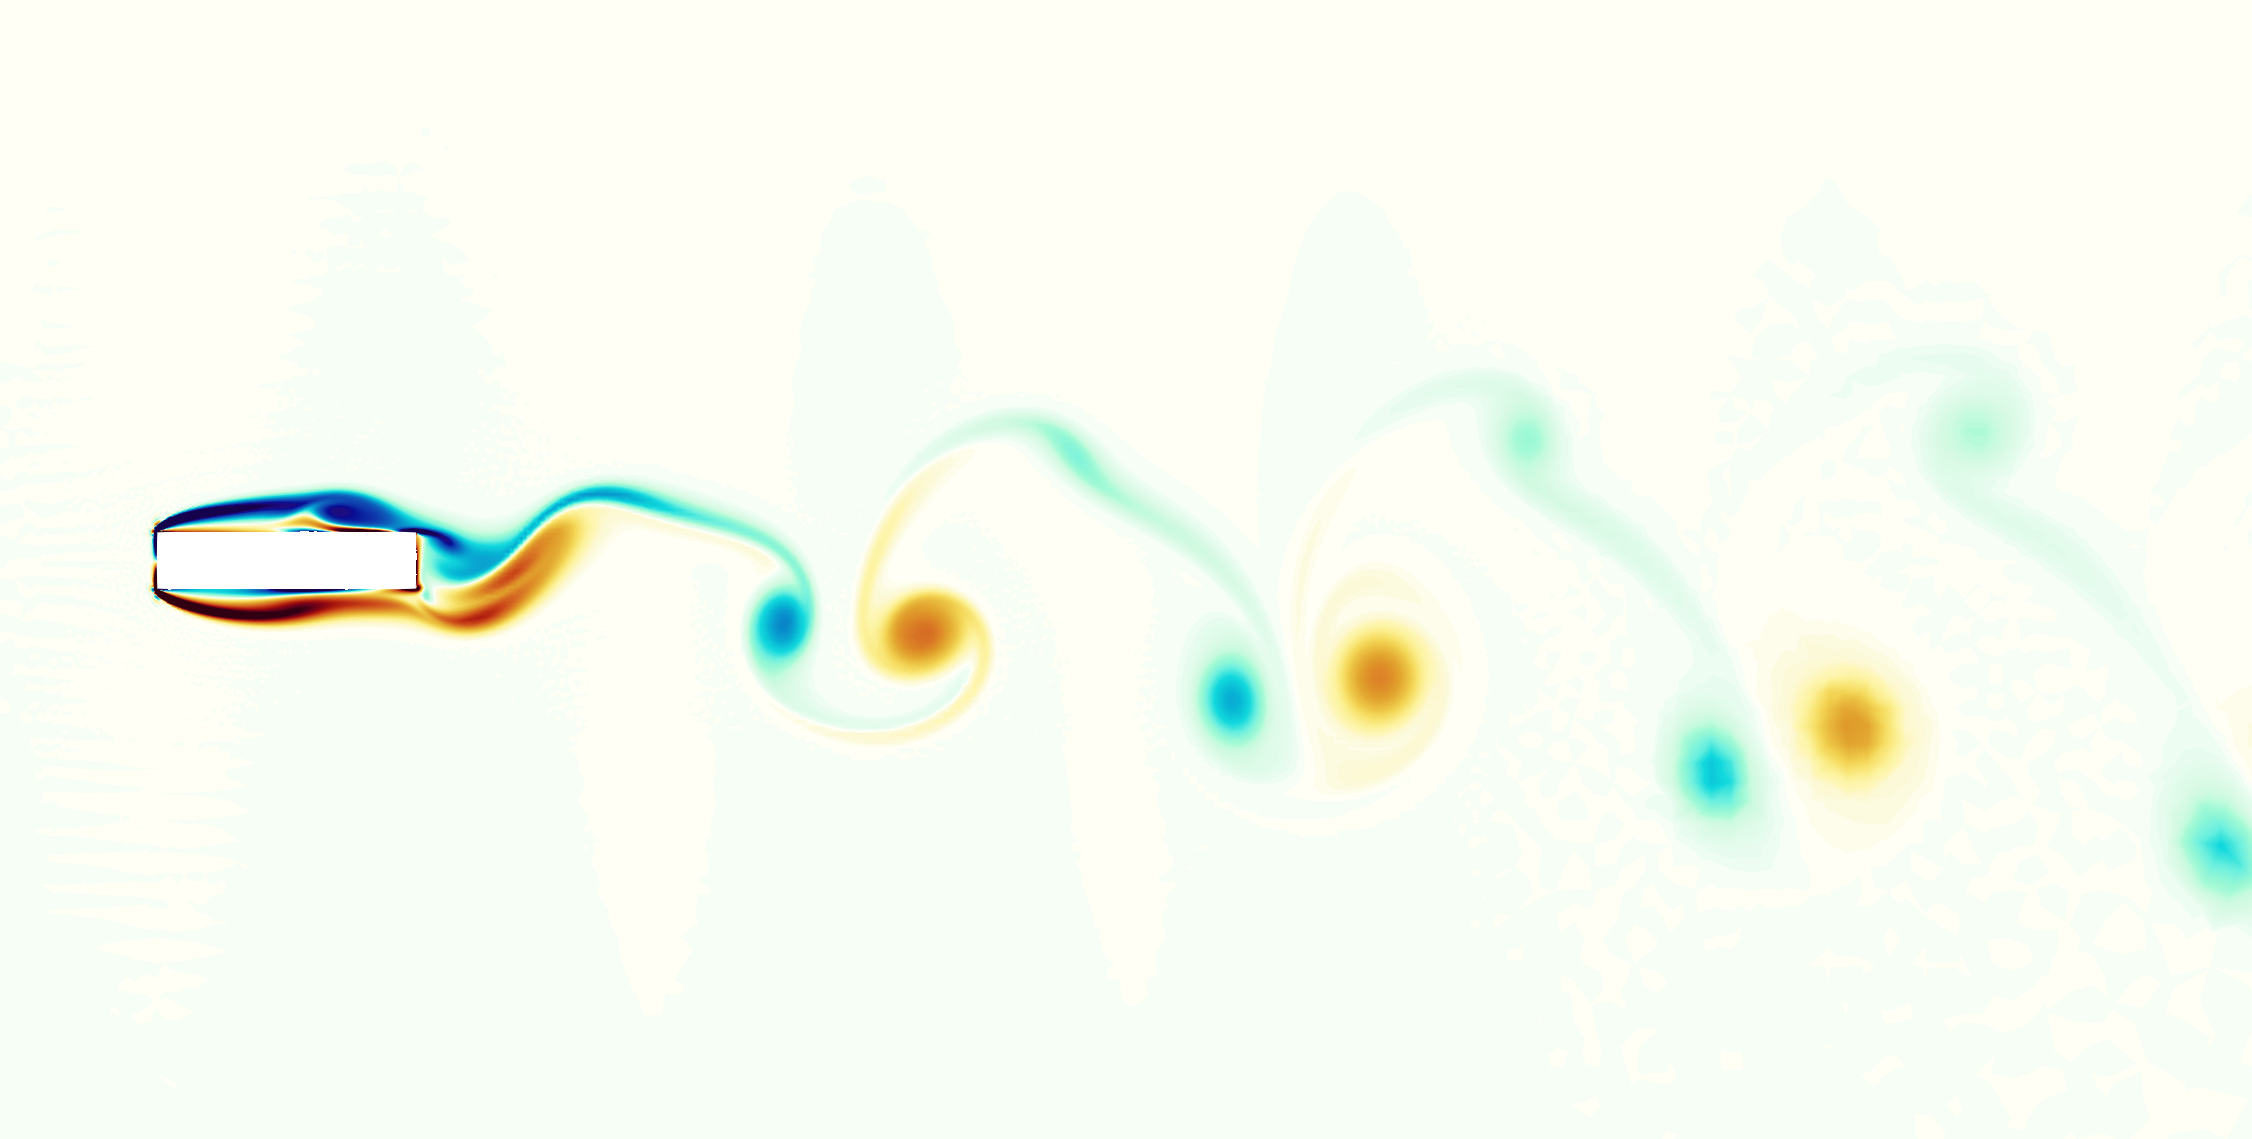
\includegraphics[trim={0 100 0 100},clip,width=0.49\textwidth]{./fig/AR4p5/vort_Re450_25.png}
  \caption{Instantaneous snapshots for $\AR=4$ at $Re=425$ (top left) and $Re=450$ (top right), and $\AR=4.5$ at $Re=430$ (bottom left) at $Re=450$ (bottom right).}
  \label{fig:snap_ar4_ar4p5}
\end{figure}

 The non linear simulations show that as $Re$ increases ($Re = Re_{c2}$) the 2D periodic base flow becomes unstable to two-dimensional perturbations and undergoes a synchronous bifurcation which leads to a flow having the same periodicity, but with a slanted wake. This is visualised in figure \ref{fig:snap_ar4_ar4p5} that show the vorticity field of instantaneous snapshots at different $Re$. For $Re< Re_{c2}$ (left panels) the wake is aligned with the $x$ axis, and characterised by the usual alternating shedding of vortices with positive/negative vorticity along the $y=0$ line. This flow regime is detailed in \cite{chiarini-quadrio-auteri-2022}, and here it is only briefly characterised for completeness. At these parameters flow dynamics is dominated by the LE vortex shedding, and a single vortex is placed at each time over the lateral sides of the cylinder. The LE vortices are advected downstream and, when they cross the TE, an hyperbolic stagnation point arises and a new TE vortex with vorticity of opposite sign is shed from the opposite side \citep{chiarini-quadrio-auteri-2022}. Here the passage of the LE vortex over the TE corner is in phase with the generation of a new TE vortex from the oppsite side of the cylinder. The relative phase at which positive (negative) LE vortices cross the TE and negative (positive) TE vortices are shed in the wake changes slightly changes with $\AR$, explaining the differences in the wake between the $\AR=4$ and the $\AR=4.5$ cases. For $\AR=4$ the LE vortices in the wake are weaker. When the Reynolds number is increased beyond $Re_{c2}$ and the flow bifurcates, the flow looses its (average) symmetry with respect to an inversion of the $y$ axis and exhibits a slanted wake. In this case, indeed, the vortex monopoled are not placed along the $y=0$ line, but they deviate apart. For $\AR=4$ this is observed for $Re \gtrapprox 435$, while for $\AR=4.5$ for $Re \gtrapprox 417.5$. Clearly, the top/bottom direction of the slanted wake changes with the initial conditions and depends on the spatial structure of the initial perturbation.

\begin{figure}
  \centering
  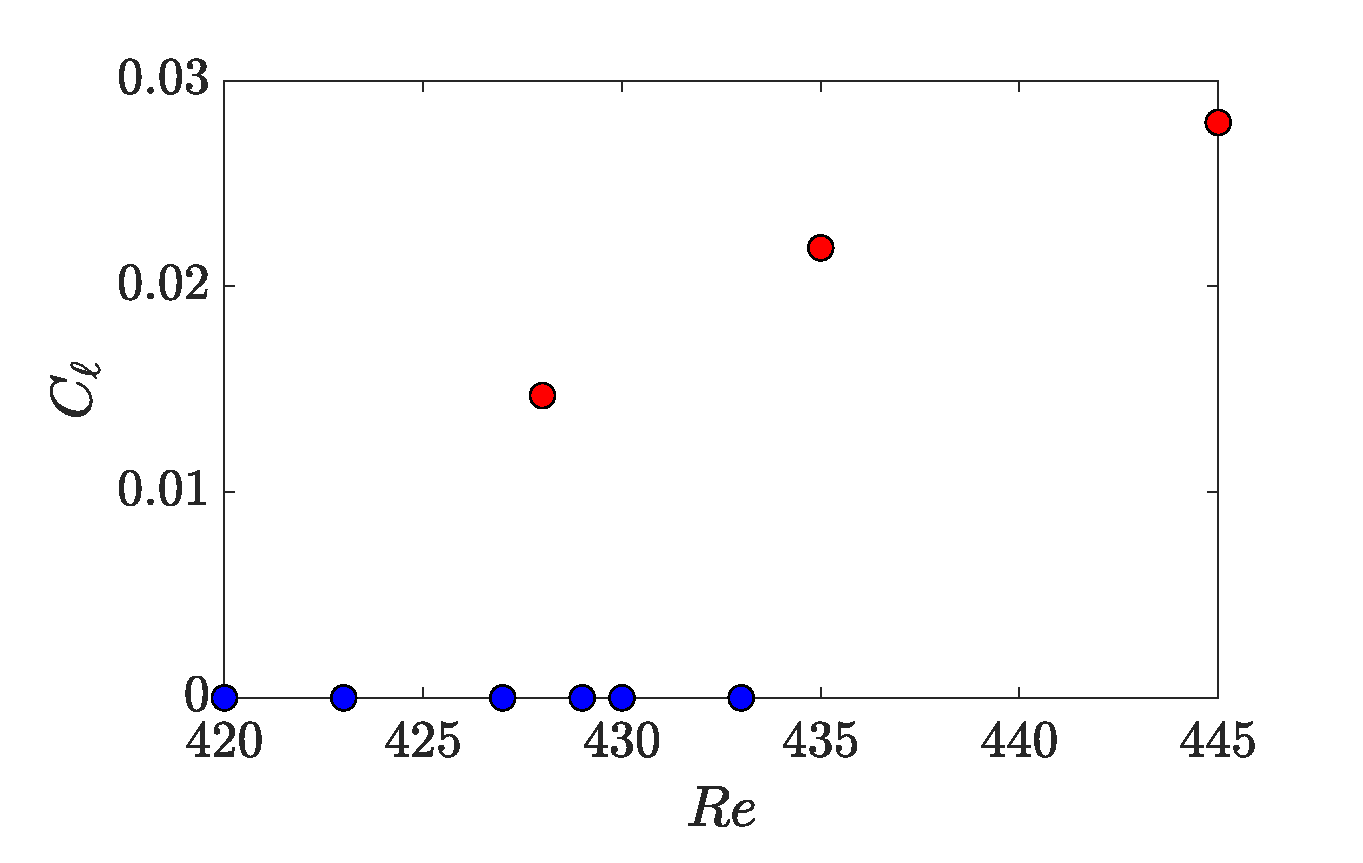
\includegraphics[width=0.49\textwidth]{./fig/AR4_Cl_Re.eps}
  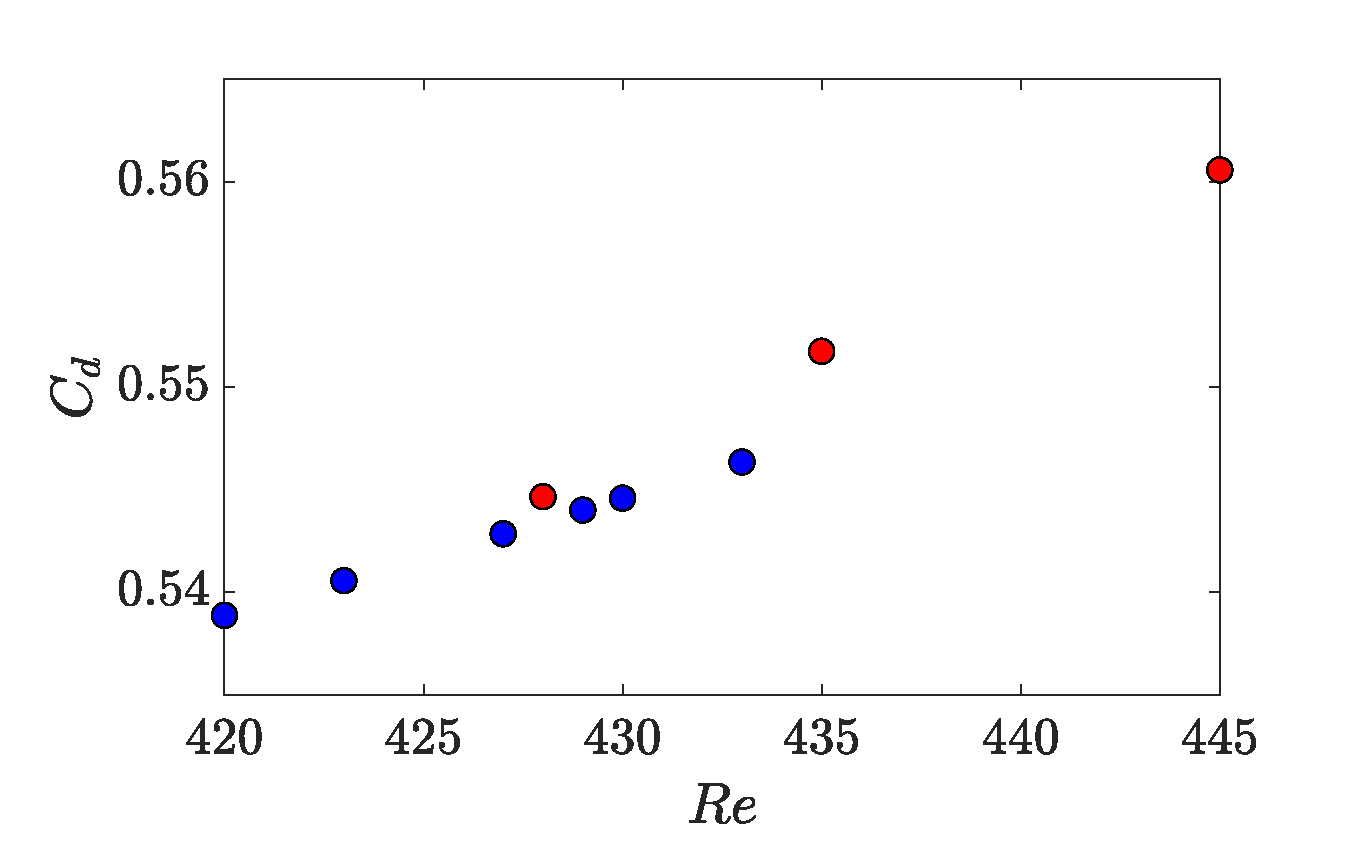
\includegraphics[width=0.49\textwidth]{./fig/AR4_Cd_Re.eps}
  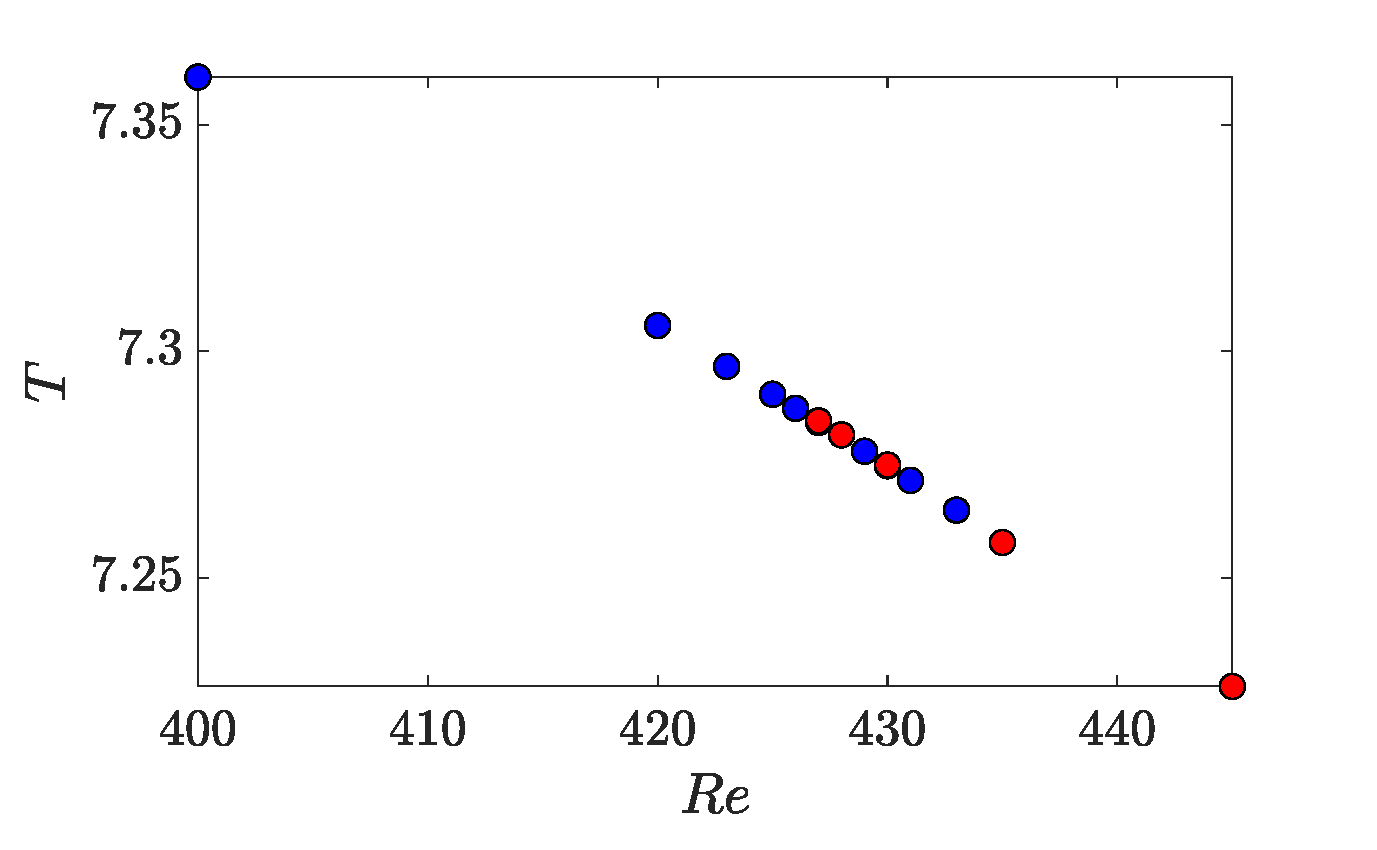
\includegraphics[width=0.49\textwidth]{./fig/AR4_T_Re.eps}
  \caption{Dependence of $C_\ell$, $C_d$ and $T$ on the Reynolds number $Re$. XX REPLACE WITH $\AR=4.5$XX}
  \label{fig:Cl-Cd-AR4}
\end{figure}
%
Figure \ref{fig:Cl-Cd-AR4} illustrated the dependence of the aerodynamic forces $C_\ell$ and $C_d$ and of the flow period $T$ on $Re$. Note that for $Re>Re_{c2}$ the unstable straight wake is stabilised by means of the BoostConv algorithm, As expected by the flow symmetries, $C_\ell=0$ for $Re \le Re_{c2}$ and $C_\ell \neq 0$ for $Re > Re_{c2}$. On the other sides, the aerodynamic drag $C_d$ increases with $Re$ in both regimes, but it increases faster in the slanted configuration. Figure \ref{fig:Cl-Cd-AR4}(c) shows that this bifurcation is og synchronous nature, as the value of $T$ collapse to the same line for both configurations showing a monotonous decrease as $Re$ increases.

\subsubsection{Linear stability analysis}
\begin{figure}
\centering
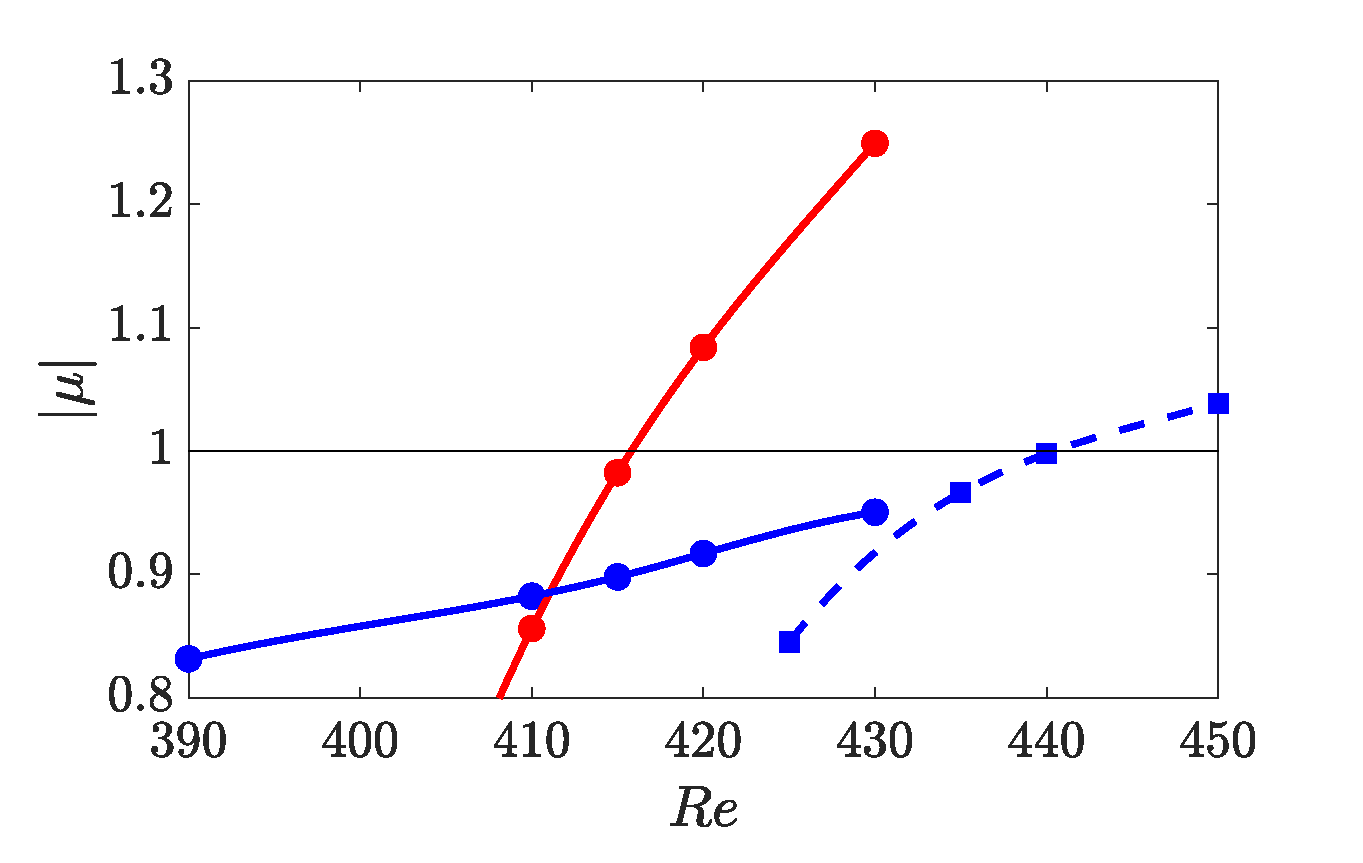
\includegraphics[width=0.49\textwidth]{./fig/AR4p5/multipliers_2D.eps}
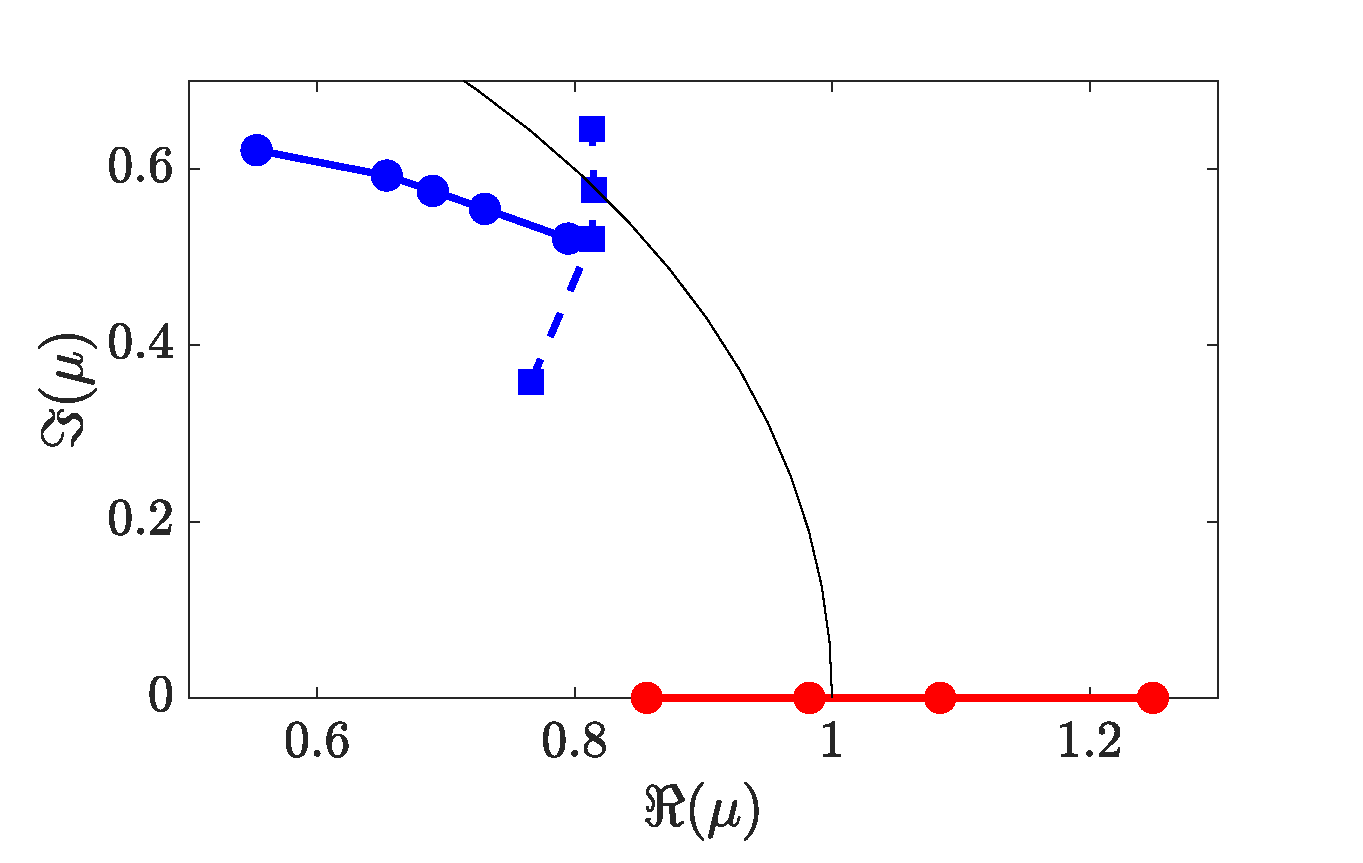
\includegraphics[width=0.49\textwidth]{./fig/AR4p5/multipliers_2D_b.eps}
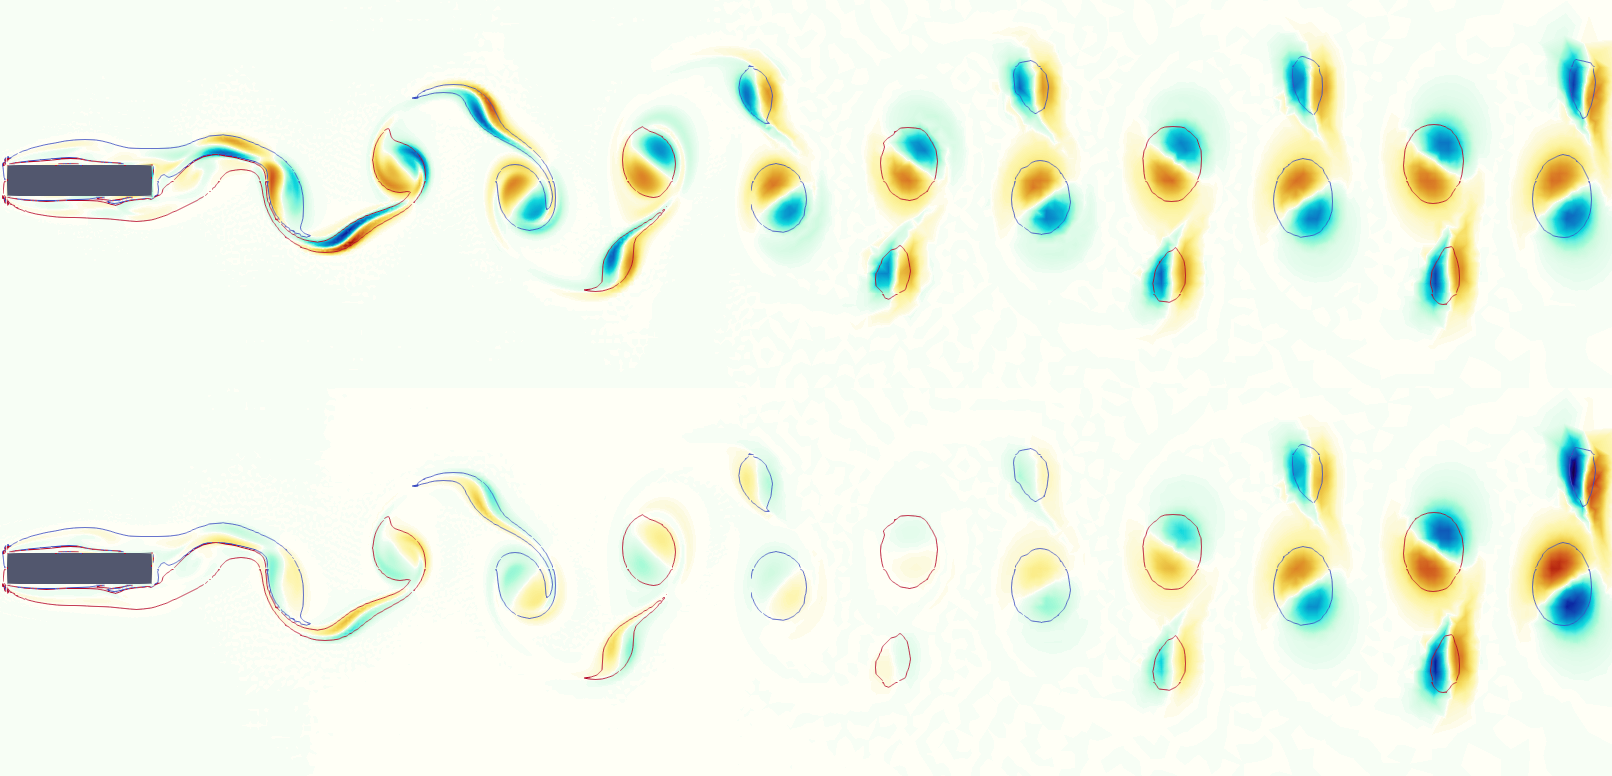
\includegraphics[width=0.7\textwidth]{./fig/AR4p5/omegaz_beta0_Re430_AB.png}
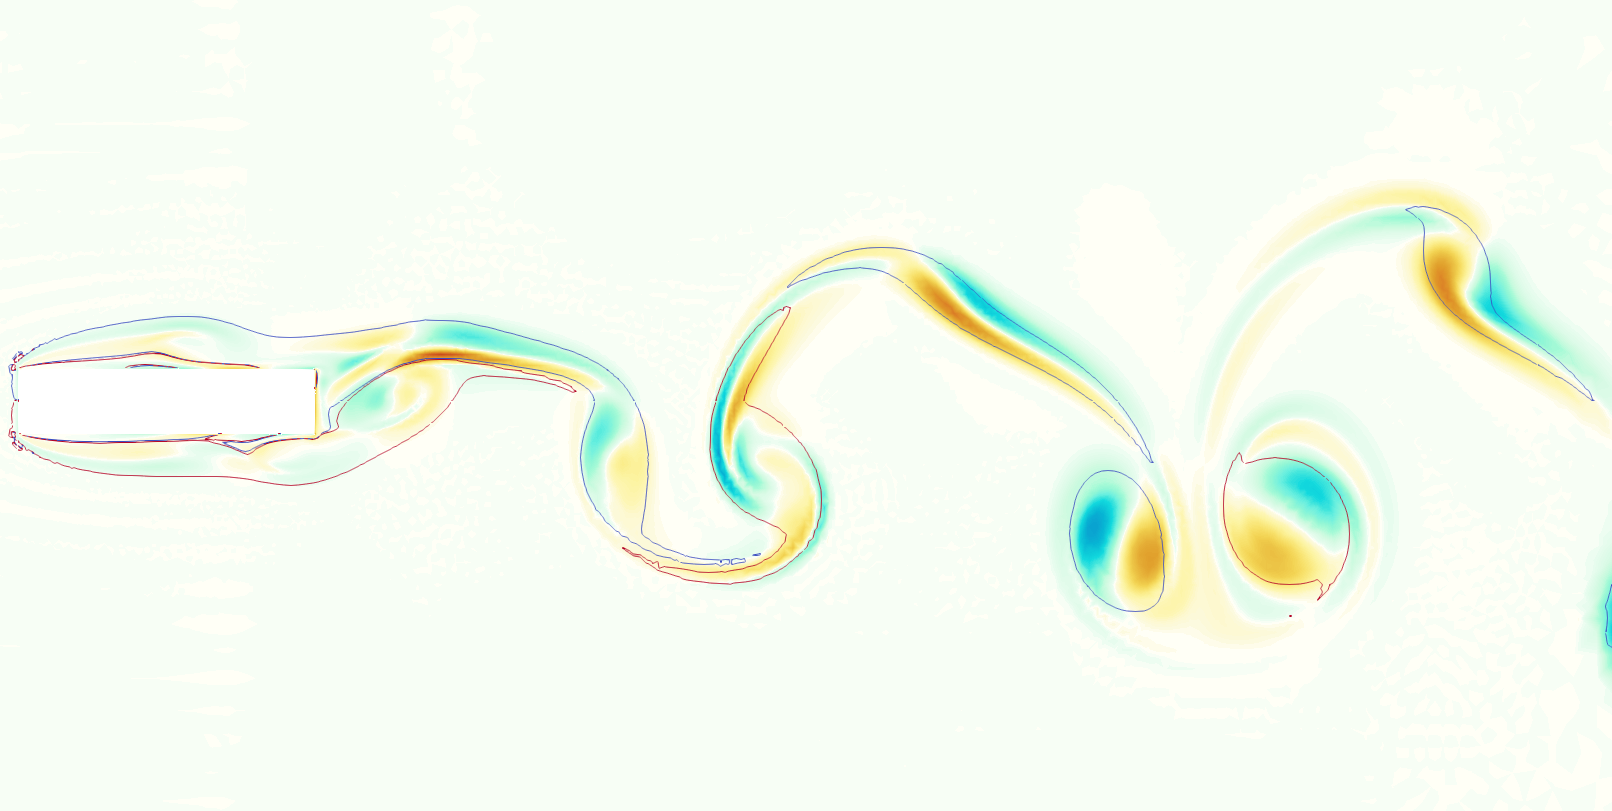
\includegraphics[width=0.7\textwidth]{./fig/AR4p5/Floqetmode_beta_0_Re450_AR4p5.png}
\caption{$2D$ bifurcation of the periodic flow past a rectangular cylinder with $\AR=4.5$. Top: Multipliers associated with the straight (solid) and slanted (dashed) wake for $\AR=4.5$. The left panel plots $|\mu|$ as a function of $\beta$. The red colour refers to real and positive multipliers, while the blue colour refer to complex mutlpliers. The right panel shows the dependence of $\Re(\mu)$ and $\Im(\mu)$ on $Re$. Note that the slanted wake is the results of the synchronous instability described by the red branch. Once the wake becomes slanted a new branch with complex conjugate multipliers arises that becomes unstable at $Re \approx 450$. Centre: Floquet modes associated with the straight wake; the colours are for the spanwise vorticity and the above and bottom panel refer to the red and blue branches respectively. Bottom: Floquet mode associated with the blue branch of the slanted wake.}
\label{fig:AR4p5_modes_Re430_beta0}
\end{figure}

To investigate the origin of this phenomenon, we have studied the linear stability of the straight wake to 2D ($\beta=0$) perturbations, using Floquet theory. We have looked at both $\AR=4$ and $\AR=4.5$, but for brevity we report only the results for the latter aspect ratio. Figure \ref{fig:AR4p5_modes_Re430_beta0}(a-b) shows with straight lines the multipliers associated with the straight wake. The red colour refers to synchronous perturbations, i.e. real and positive multipliers. The blue colour, instead, refers to complex conjugate multipliers i.e. to quasi-periodic modes. The red branch crosses the unit circle at $Re = Re_{c2} \approx 417.5$ (for $\AR=4$ we measure $Re_{c2} \approx 425$). The fact that $\Im(\mu)=0$ confirms that the slatend wake is the result of a synchronous global instability of the wake. The blue branch associated with the quasi-periodic mode does not become unstable in the considered range of parameters. 

To provide further details, figure \ref{fig:AR4p5_modes_Re430_beta0} shows the spanwise vorticity of the unstable Floquet mode together with isolines of the base-flow vorticity. In the wake, the unstable mode generates dipoles of spanwise vorticity that frow in space and time as they are advected downstream. A synchronisation between the base flow and the perturbation field is obseved, with the dipoles of the linear mode being centred with the base-flow vortices at all times. A dipolar perturbation of a monopolar vortex is often referred to as displacement mode \citep{brion-sipp-jacquin-2014} and is known to result in a displacement of the vorticity centroid similarly to what observed for $Re>Re_{c2}$ in figure \ref{fig:snap_ar4_ar4p5}. We consider a positive base-flow virticity monopole in the wake. Here the Floquet dipole has positive vorticity in the lower part and negative vorticity in the upper part. This superposition stregthens the lower part of the monopole and weaken the top part, resulting into a net displacement  of the monopole in the downwards direction. In the monopoles of negative base-flow vorticity, instead, the scenario is the opposite. The Floquet dipole has positive vorticity in the top part of the monopole and negative vorticity in the bottom part. This strengthens the bottom part of the monopole and weakens the top parti, resulting again into a downward shift of the monopole. This explains the vertical displacement of the vortex centroids shown in figures \ref{fig:snap_ar4_ar4p5}. We mention that this mechanism resembles that observed in \cite{jallas-marquet-fabre-2017} in the case of pitching airfoils.

For completeness, we report that the slanted wake is then unstable to 2D perturbations of quasi-periodic nature. However, as shown in the following this is a secondary bifurcation of the slanted-wake base flow, as the flow becomes three-dimensional at lower $Re$.

\subsubsection{Non linear effects}


\begin{itemize}
  \item \textcolor{blue}{ Amplitude equation non è esattamente corretta. Quel valore di A che ottengo non è esattamente la stessa amplitude che si ottiene per $\hat{\bm{u}}_1$ quando si fa WNL con un'espansione alle scale multiple. Infatti in quel caso il campo di velocità dovrebbe essere $\bm{u} = \bm{u}_0 + \epsilon A(T) \bm{u}_1 ..$ dove nei termini successivi (per esempio $\bm{u}_2$) ci sono anche correzioni al flusso base. Quindi, fai attenzione non è esattamente la stessa cosa. }
  \item \textcolor{blue}{ Possiamo fare un'espansione alle scale multiple per trovare che forma ha questa amplitude equation? Possiamo fare veramente and una WNL su questa biforcazione o non è possibile? }
  \item \textcolor{blue}{ Leggi bene anche gli articoli di Barkley \& Hendersson }
\end{itemize}


\begin{figure}
  \centering
  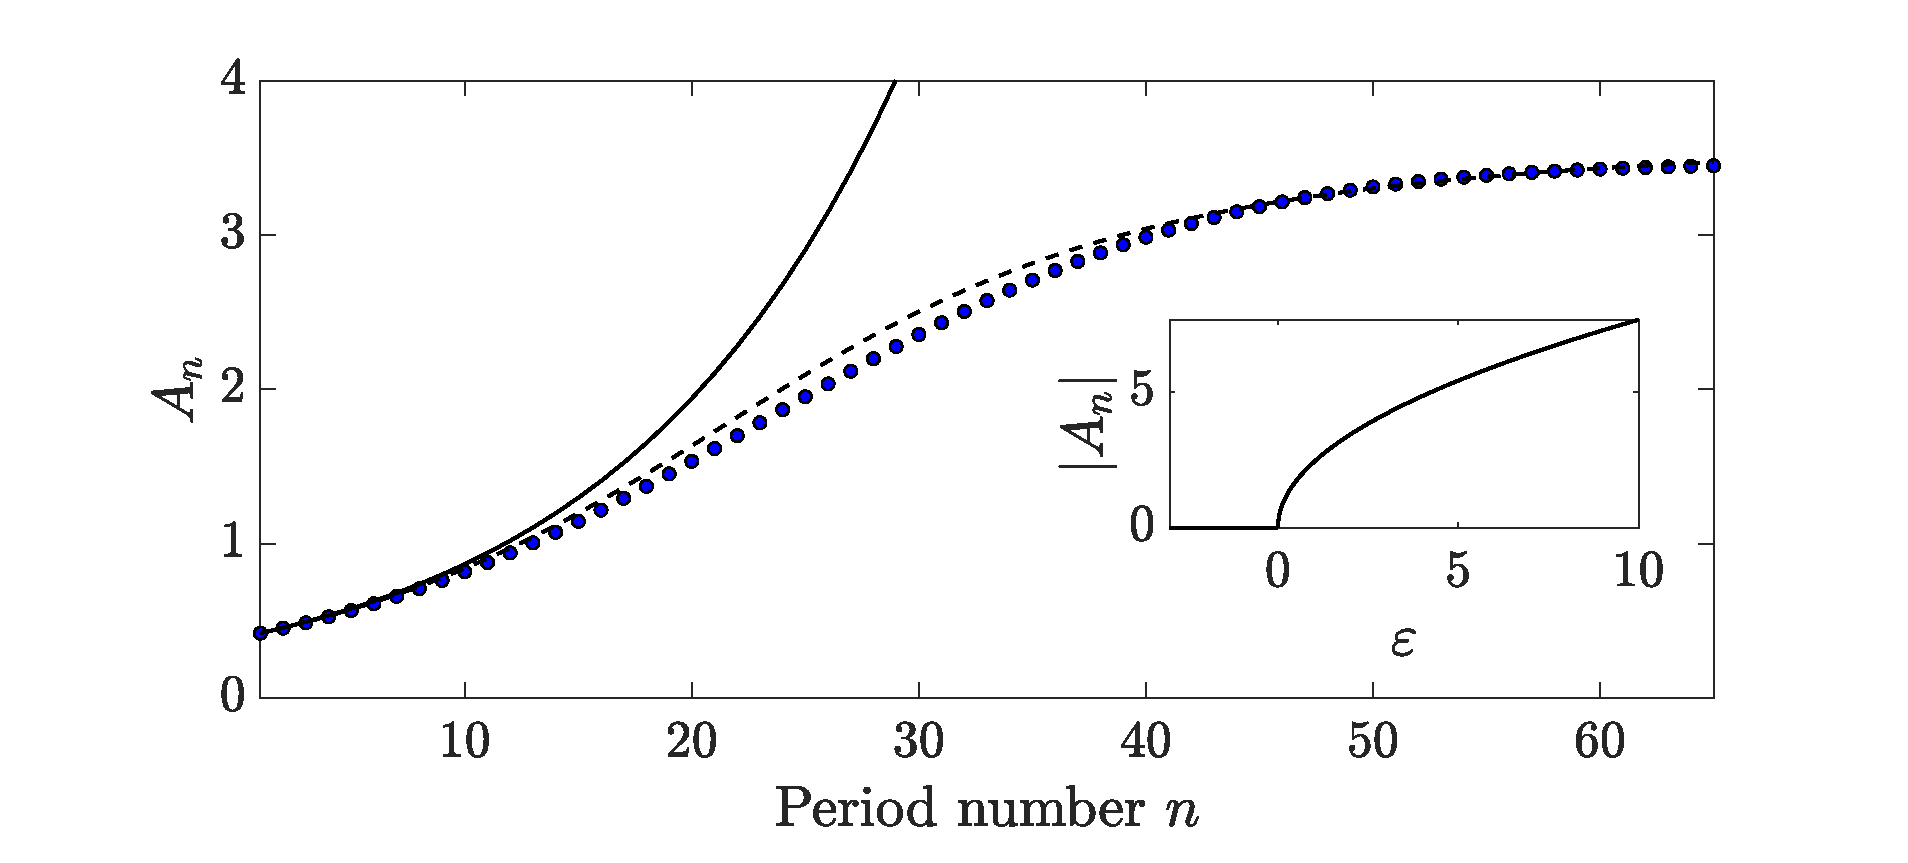
\includegraphics[width=0.7\textwidth]{./fig/AR4p5/Nlgrowth_Re420.eps}
  \caption{Nonlinear growth of the 2D perturbation to the wake near the secondary instability threshold for $\AR=4.5$ and $Re=420$. Top: the blue circles are the amplitude of $A_n$ evaluated from simulations of the full Navier--Stokes equations at $Re=420$. The solid line shows the prediction $A_{n+1} = \mu A_n$, while the dashed line shows the prediction $A_{n+1} = ( \mu + \alpha_1 A_n + \alpha_2 A_n^3 ) A_n$, with $\alpha_1 = -0.01114$ and $\alpha_2 = 0.000359$. The inset shows the bifurcation diagram.}
  \label{fig:ar4p5_nnl}
\end{figure}

The linear stability analysis detailed in the previous section explains the onset of the instability. However, it does not provide any description of the resulting asymmetric limit cycle. Indeed, linear theory is enough to predict the critical Reynolds number $Re_{c2}$, but non linear effects must be included to understand the dynamics of the flow beyond the mere onset of the linear instability. 

Indeed, close to a critical point we can reduce the wake dynamics to that of a discrete-time dynamical system \citep{henderson-barkley-1996,henderson-1997}. We thus start writing the complete flow field as
%
\begin{equation}
  \bm{u}(\bm{x},t) =  U \bm{u}_0(\bm{x},t) + A(t) \bm{u}_1(\bm{x},t),
\end{equation}
%
where $|| \bm{u}_0 || = 1 $ and $|| \bm{u}_1 || = 1$. We then discretise time, only considering the state of the system at discrete times $t_n$, representing one pass through the shedding cycle ($t_{n+1} = t_n + T$) to obtain
%
\begin{equation}
  \bm{u}(\bm{x},t_n) = U \bm{u}_0(\bm{x},t_n) + A_n \bm{u}_1(\bm{x},t_n).
\end{equation}
%
As a result, the flow dynamics if largely described by the discrete-time evolution of the amplitude $A_n \equiv A(t_n)$, and the discrete evolution of $\bm{u}_1(\bm{x},t_n)$ characterises the influence of the non linearity on the perturbation.

For the nonlinear classification of the instability, we consider the normal form for a pitchfork bifurcation of a discrete-time dynamical system, i.e. 
%
\begin{equation}
  A_{n+1} = \left( \mu  + \sum_{j=1}^\infty \alpha_j A_n^{2j} \right) A_n,
\end{equation}
%
where $A_n$ corresponds to the real amplitude of the bifurcating flow at period $n$ and the coefficient $\alpha_1$ is called the Landau constant. If $\alpha_1 <0$ the instability is a supercritical or soft bifurcation. If $\alpha_1>0$ the instability is a subcritical or hard bifurcation. When the bifurcation is supercritical (as in the present case) the limiting amplitude can be determined by considering only the first two terms of the expansion. Substituting $\mu = 1 + \mu' \epsilon$, where $\epsilon \equiv (Re - Re_{c2})/Re_{c2}$ and $\mu' = \text{d}\mu/\text{d}\epsilon$ the finite-amplitude states are given by
%
\begin{equation}
  |A|^2 =- \mu' \epsilon / \alpha_1.
\end{equation}

To deterimine the nonlinear character of the secondary instability we thus performed non linear simulations at $Re \approx Re_c$, following the evolution of the velocity field in the form $\bm{u}_1 + \bm{u}_{nl}$, where $\bm{u}_{nl}$ is the nonlinear perturbation, and using $\bm{u}_{nl} = \hat{\bm{u}}_1$ as initial condition. The amplitude $A_n$ of the perturbation after $n$ shedding period is determined as
%
\begin{equation}
  |A_n|^2 = \frac{1}{\Omega U_\infty^2} \int_{\Omega} | \bm{u}_{nl,n} |^2 \text{d} \Omega
\end{equation}
%
The nonlinear character of the instability is thus evaluated after estimating the values of the $\alpha_j$ coefficients with the simulation.

Figure \ref{fig:ar4p5_nnl} shows the results for $\AR=4.5$ at $Re=420$ ($\epsilon \approx 0.01$), but the same results have been obtained for $\AR=4$. Starting from a small perturbation the instability saturates after $\mathcal{O}(50)$ shedding periods. At this $Re$ the linear growth of the perturbation is $\mu \approx 1.083$. However, the amplitude $A_n$ drops below the exponential growth curve near saturation. The estimated value of the Landau constant is $\alpha_1 \approx - 0.011 <0$, indicating that the instability is supercritical. This is consistent with the $C_l(Re)$ diagram shown in figure \ref{fig:Cl-Cd-AR4}.

\begin{figure}
  \centering
  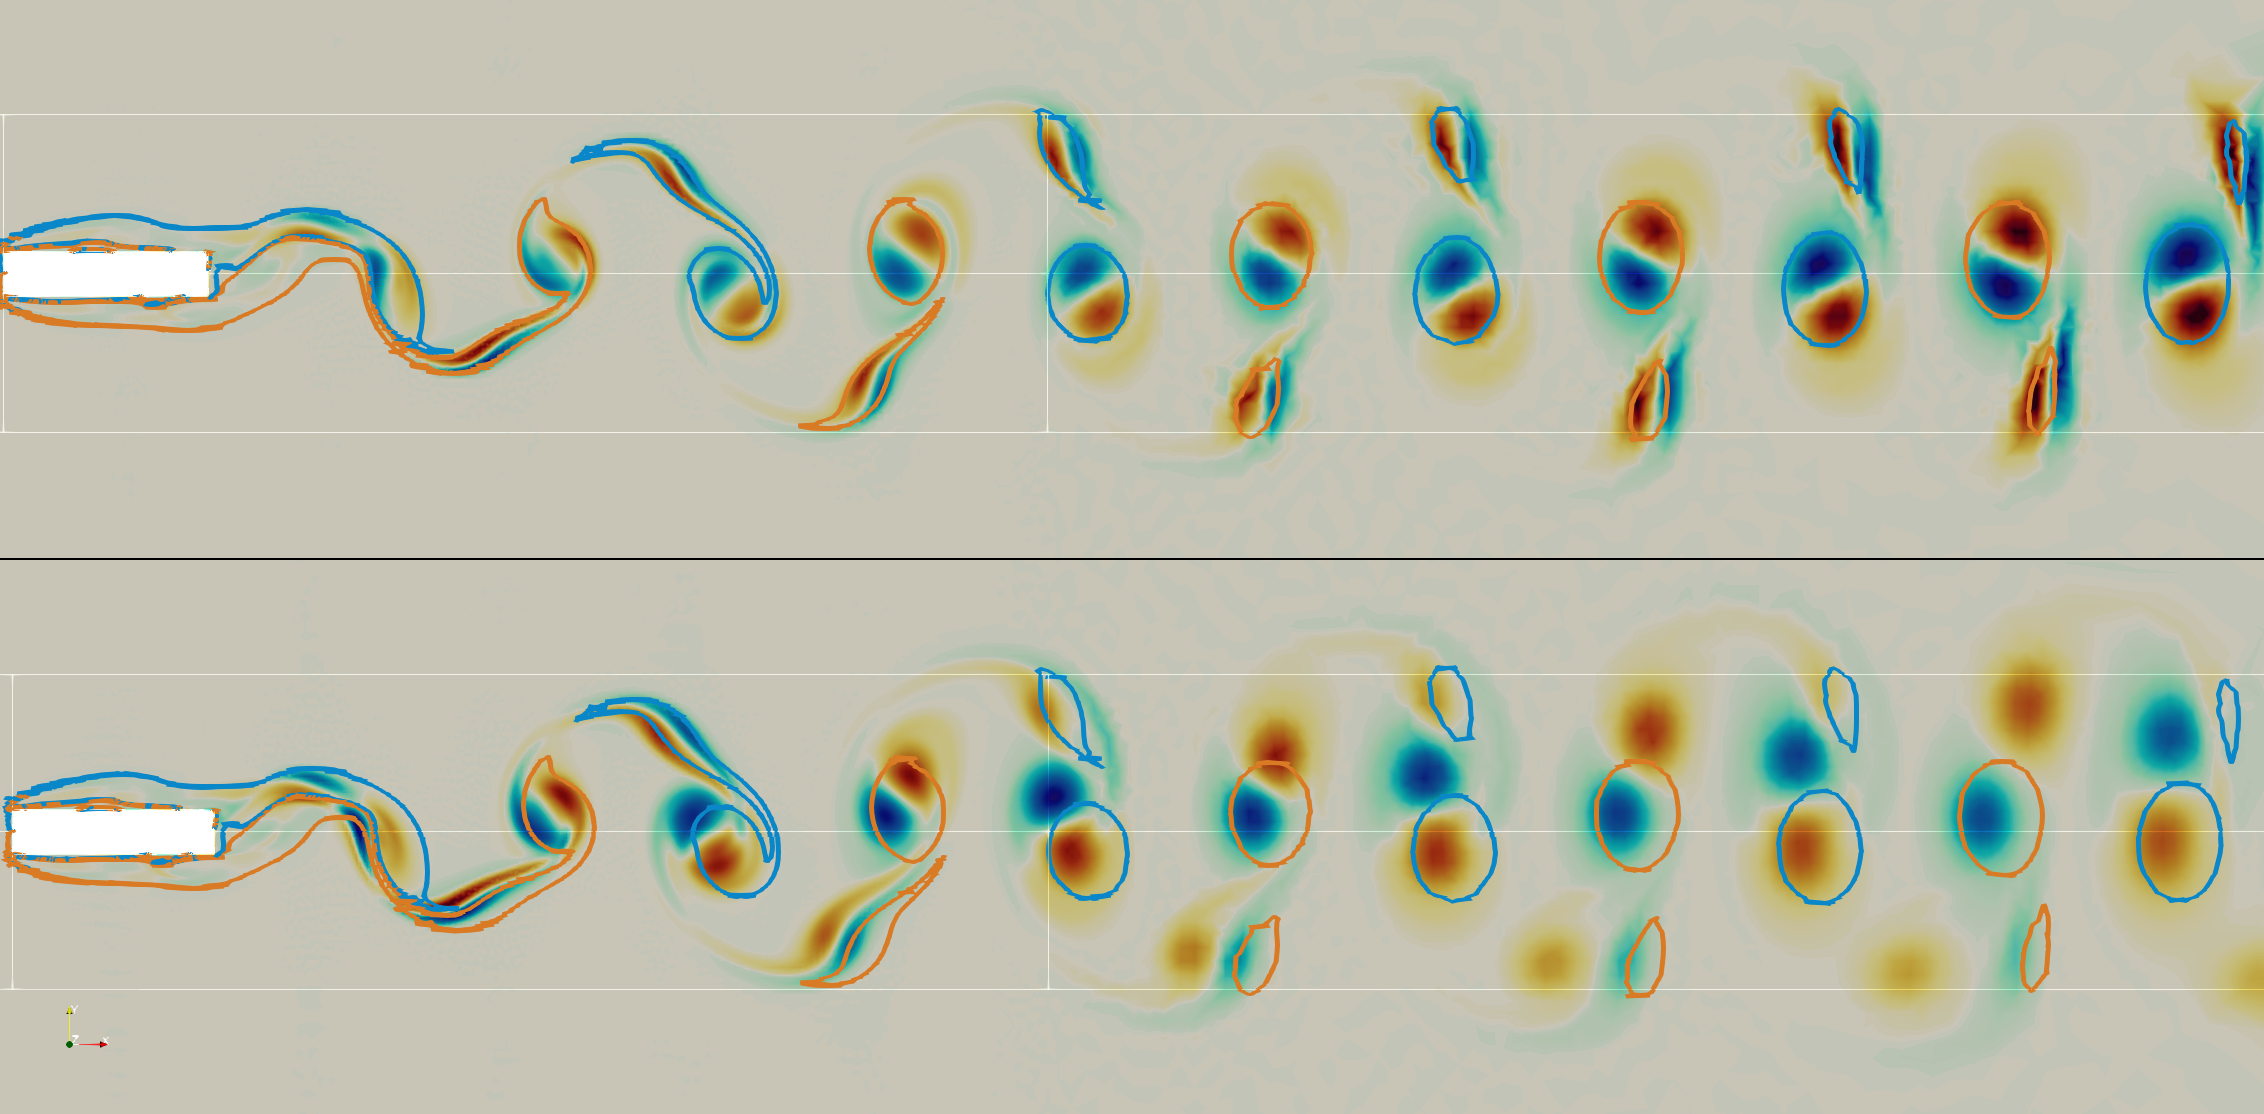
\includegraphics[width=0.9\textwidth]{./fig/AR4p5/nl_Re420.png}
  \caption{Perturbation field for $\AR=4.5$, $Re=420$ and $\beta=0$. Top: linear perturbation. Bottom: non linear perturbation.}
  \label{fig:pert-nl}
\end{figure}

Figure \ref{fig:pert-nl} shows snapshots of the linear and non linear perturbations. As mentioned previously, the linear perturbation is essentially an array of dipolar structures aligned with the $x$ axis and centred in the monopolar structures of the base flow. We note that just downstream the TE the nonlinear perturbations resemble the linear ones, suggesting that the nonlinear effects are negligible in the near wake. When moving downstream the influence of the nonlinearity becomes evident. The nonlinear perturbation shows a specific pattern such that the dipolar structure of the perturbation field are not centred with the monopolar structures of the base flow. The perturbation dipoles indeed expand in the cross-flow direction and they organise in such a way that in correspondence of the base-flow monopolar structure the perturbation field has vorticity of opposite sign, to make the straight wake to disappear in the complete velocity field.

\subsection{The 3D bifurcation}

\subsubsection{Linear stability analysis}

\begin{figure}
  \centering
  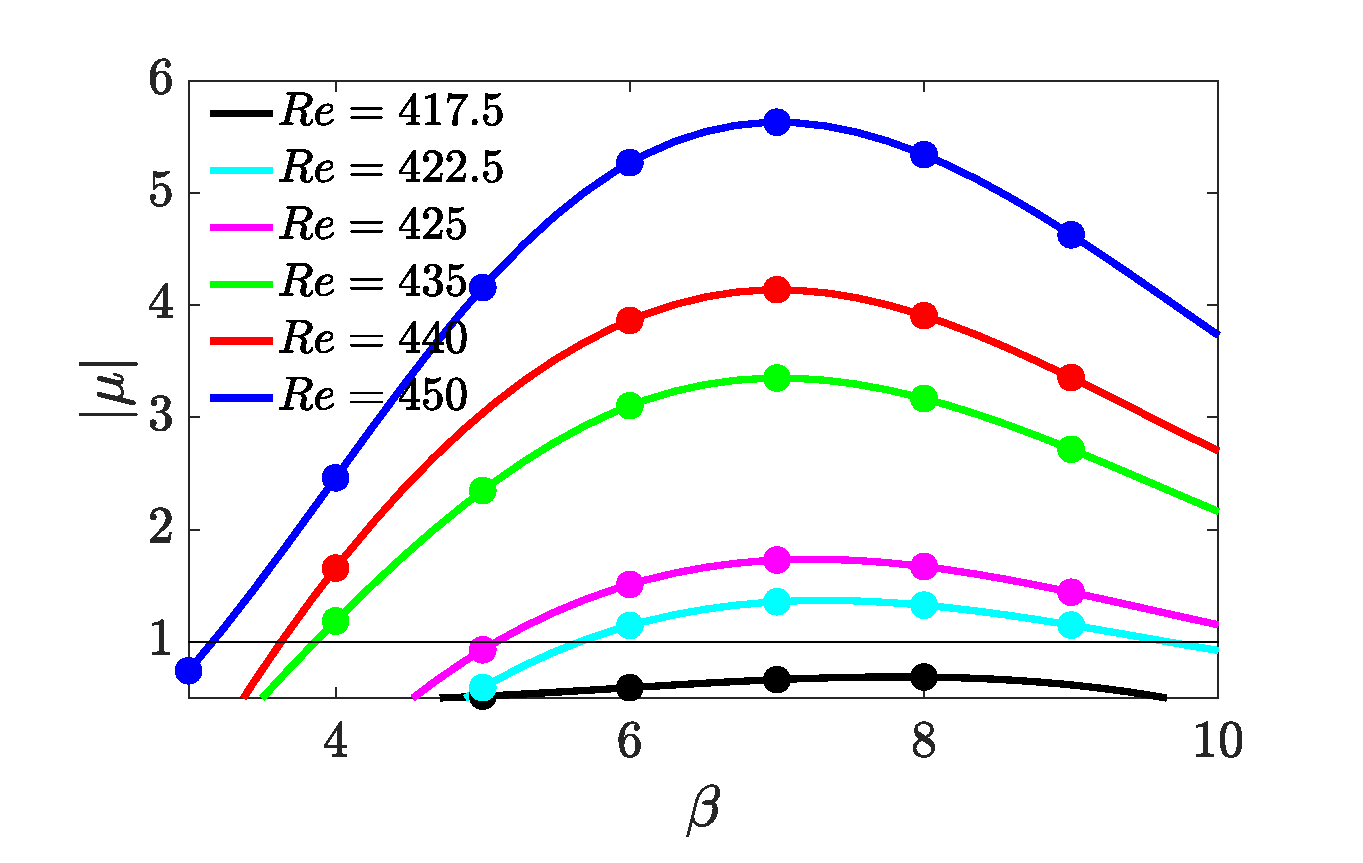
\includegraphics[width=0.49\textwidth]{./fig/AR4p5/multipliers_3D.eps}
  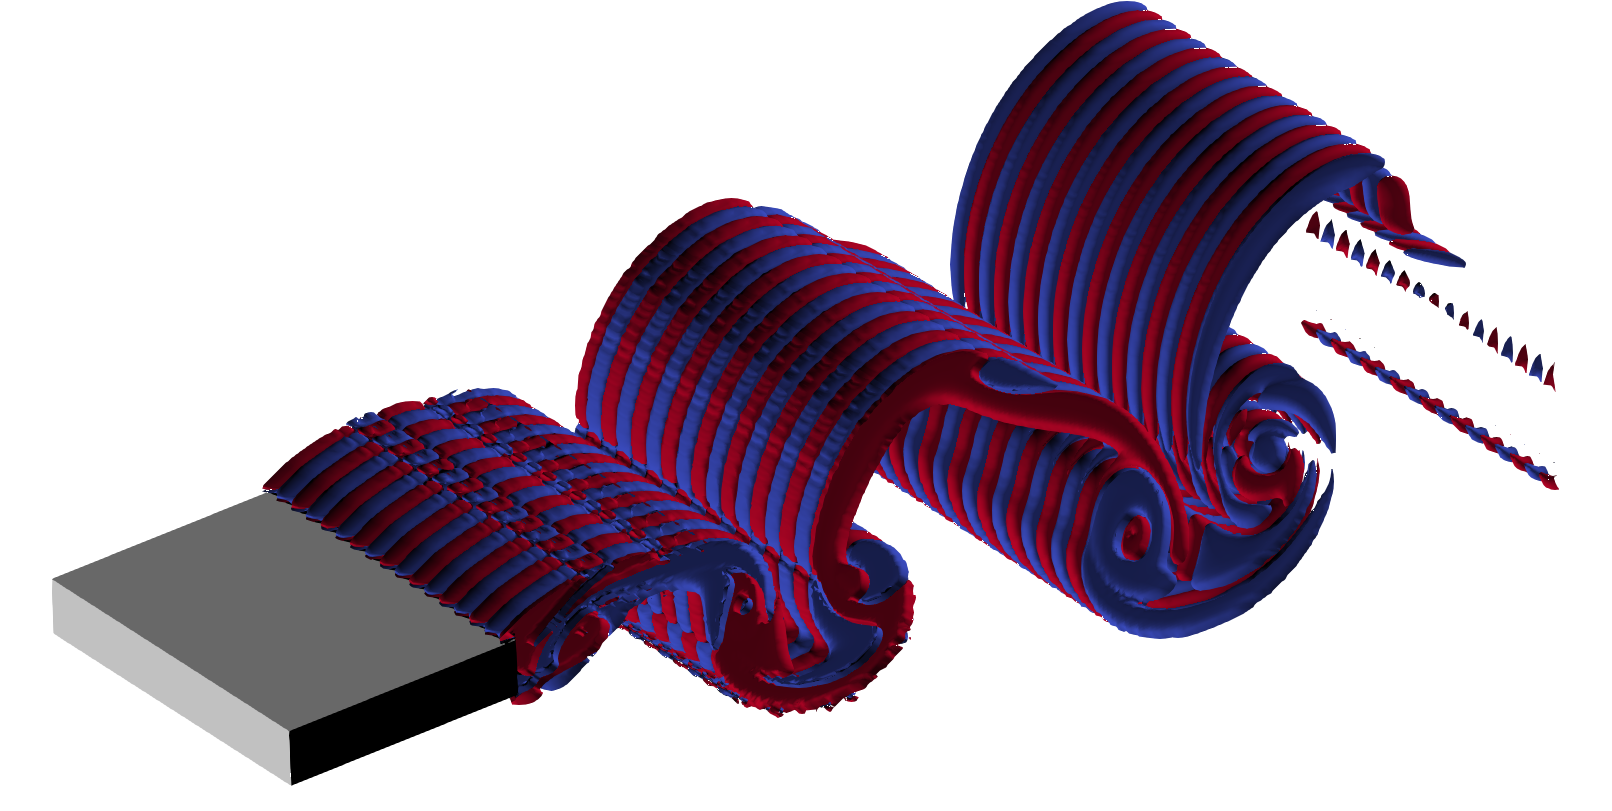
\includegraphics[trim={0 0 0 0},clip,width=0.7\textwidth]{./fig/AR4p5/Floqetmode_beta_8_Re450_AR4p5.png}  
  \caption{Three-dimensional instability for $\AR=4.5$. The flow becomes unstable to three-dimensiona perturbations once the was has bifurcated to a deflected configuration. The figure shows the dependence of the Floquet multilpiers on $Re$ and $\beta$. For all cases $\mu$ is real and negative, indicating a subharmonic bifurcation. Bottom: Imaginary part of the streamwise vorticity for $\AR=4.5$, $Re=450$ and $\beta=8$ associated with the unstable subharmonic multiplier. XX AGGIUNGIAMO QUA LA SENSITIVITA STRUTTURALE XX}
  \label{fig:mul-3d-ar4p5}
\end{figure}

For $Re \ge Re_{c2}$ the flow approaches a new limit cycle characterised by a deflected wake (see the previous section), which is strongly unstable to three-dimensional perturbations. We have investigated the linear stability of this new state using Floquet analysis. Here we focus again on $\AR=4.5$, but similar results are obtained also for $\AR=4$. Figure \ref{fig:mul-3d-ar4p5} shows the dominant Floquet multipliers for different values of $Re$ in the range $417.5 \le Re \le 450$ and for $3.5 \le \beta \le 10$. A first multiplier with $|\mu|>1$ appears for $Re = Re_{c3} \approx 420$ and $\beta=7$. The two-dimensional deflected wake remains thus stable for a very small range of $Re$. For $Re > Re_{c3}$, a band of unstable wavenumbers appears, with $\beta_{max}$ only marginally varying with $Re$. Interestingly, the growth rate shows a strong increase with $Re$ with $|\mu| \approx 2$ for $Re=425$ and $\mu\approx 9$ for $Re=450$. The unstable multipliers is real with negative real part, indicating that the periodic deflected wake is linearly unstable to 3D subharmonic perturbations. Note that such an unstable Floquet multiplier with negative real part and zero imaginary part could not exist for base flows that obey the spatio-temporal symmetry (like at lower $Re$), as demonstrated by \cite{marques-lopez-blackburn-2004,blackburn-etal-2005}. However, modes of subharmonic nature are often observed once the symmetries of the base flow are brokes, for example by introducing a non negligible incidence angle in the flow past a square cylinder \citep{blackburn-sheard-2010}.
%
Figure \ref{fig:3dmode-ar4p5}(a) shows the spatial structure of the real part of the streamwise vorticity of the subharmonic mode for $Re=450$ and $\beta=8$. The perturbation field is maximum near the vortex cores of the base flow, as for the flow past other bluff bodies, see for example \cite{thompson-leweke-williamson-2001,chaurasia-thompson-2011}. Interestingly, the perturbation field in completely localised in the wake, being almost null over the cylinder sides. Unlike the QS mode \citep{chiarini-quadrio-auteri-2022d}, this is an unstable mode of the wake and the LE vortices placed over the lateral sides of the cylinder do not play any role in the triggering mechanism. The symmetry of the much is such that the sign of the streamwise vorticity changes sign from one period to the next, in agreement with the subharmonic nature of the mode.

\begin{figure}
  \centering
  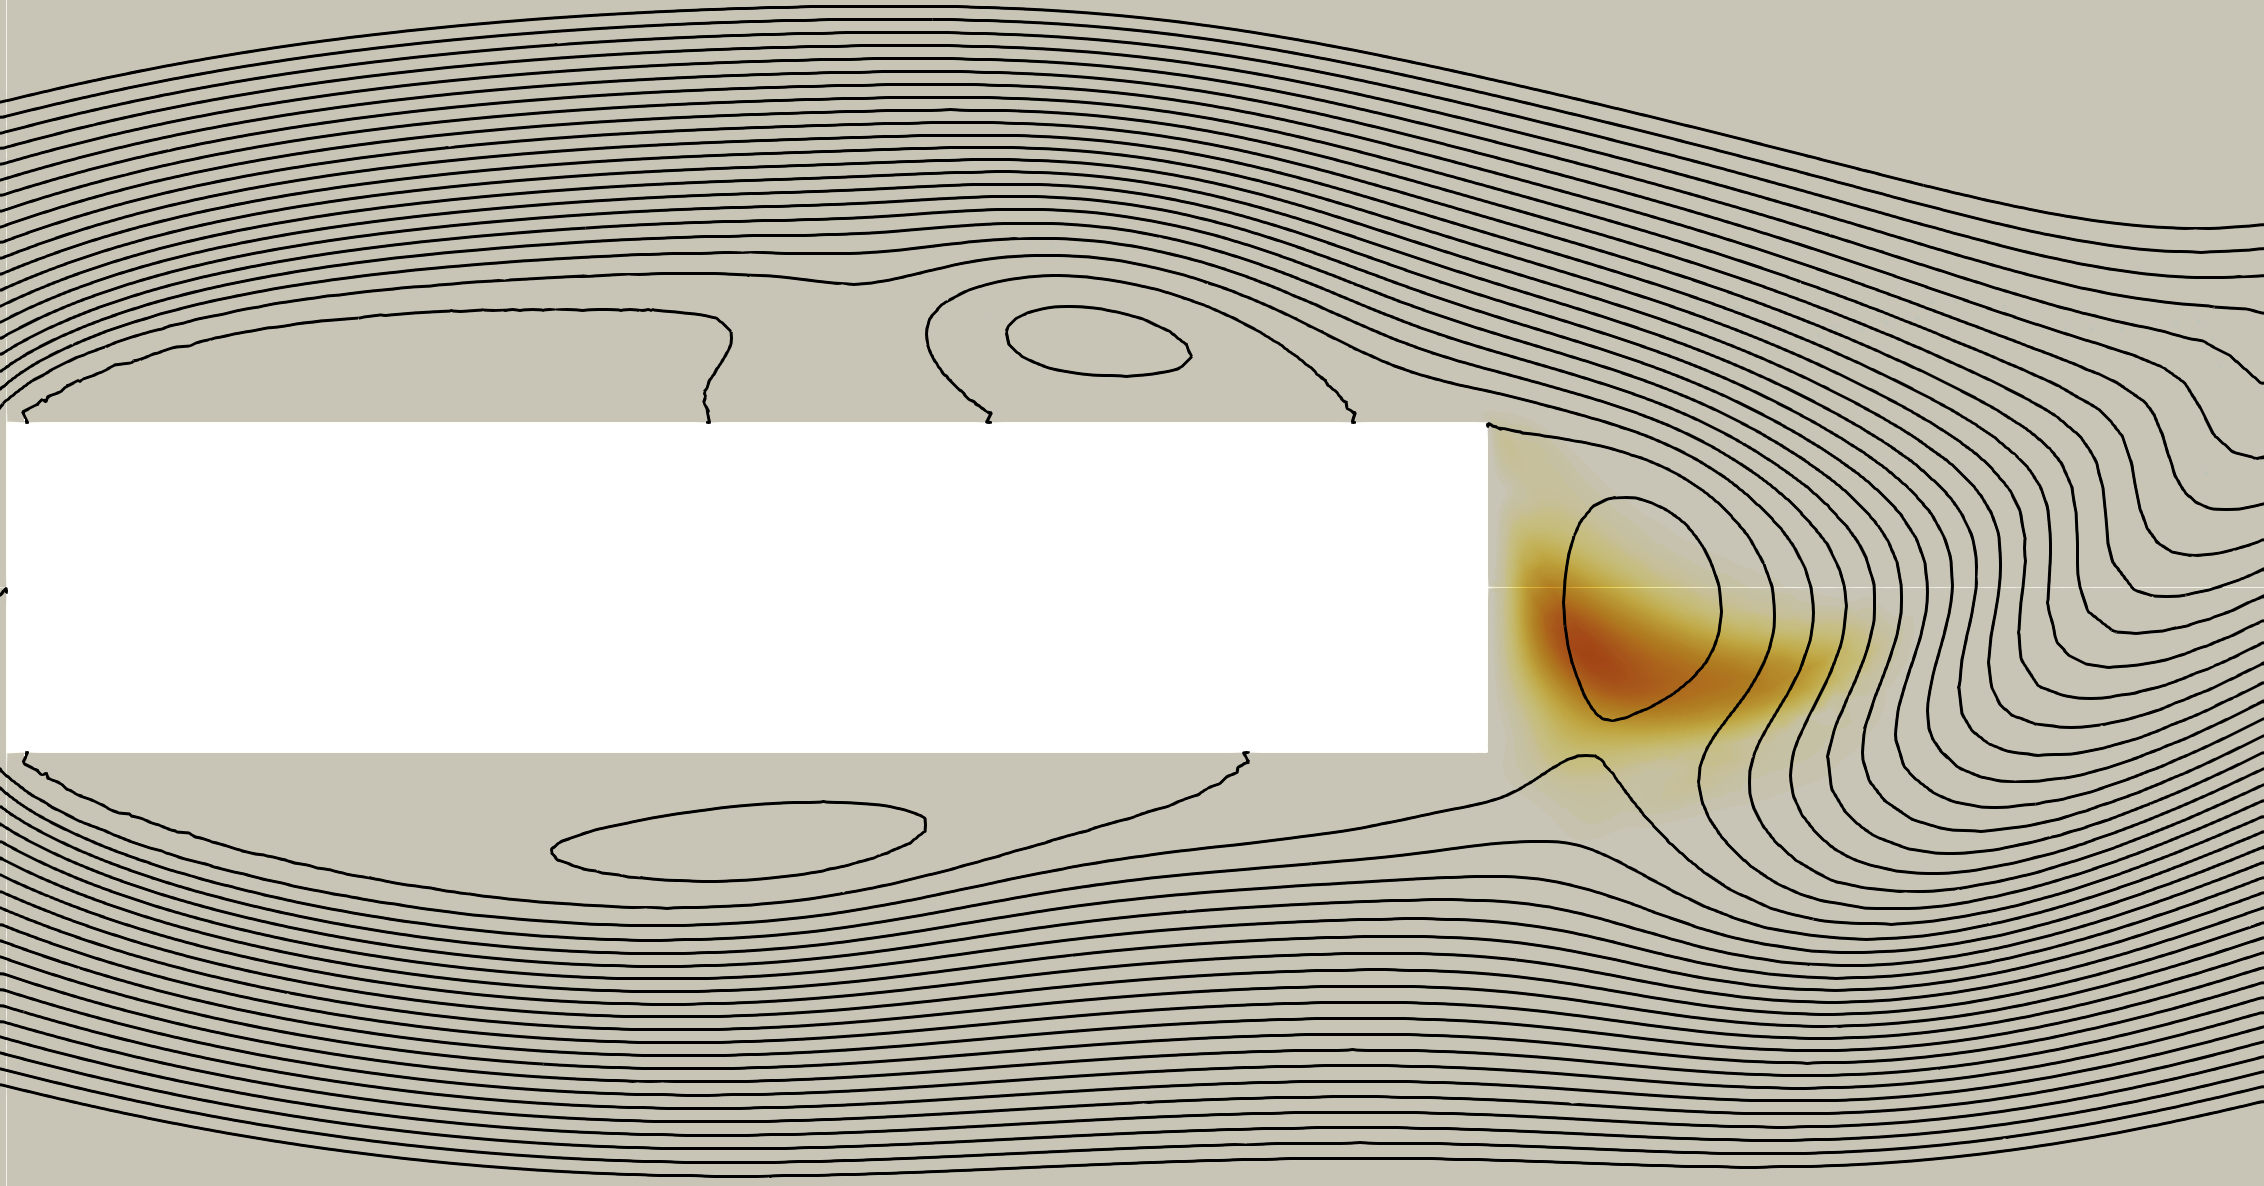
\includegraphics[width=0.49\textwidth]{./fig/AR4p5/sens3D_25.png}
  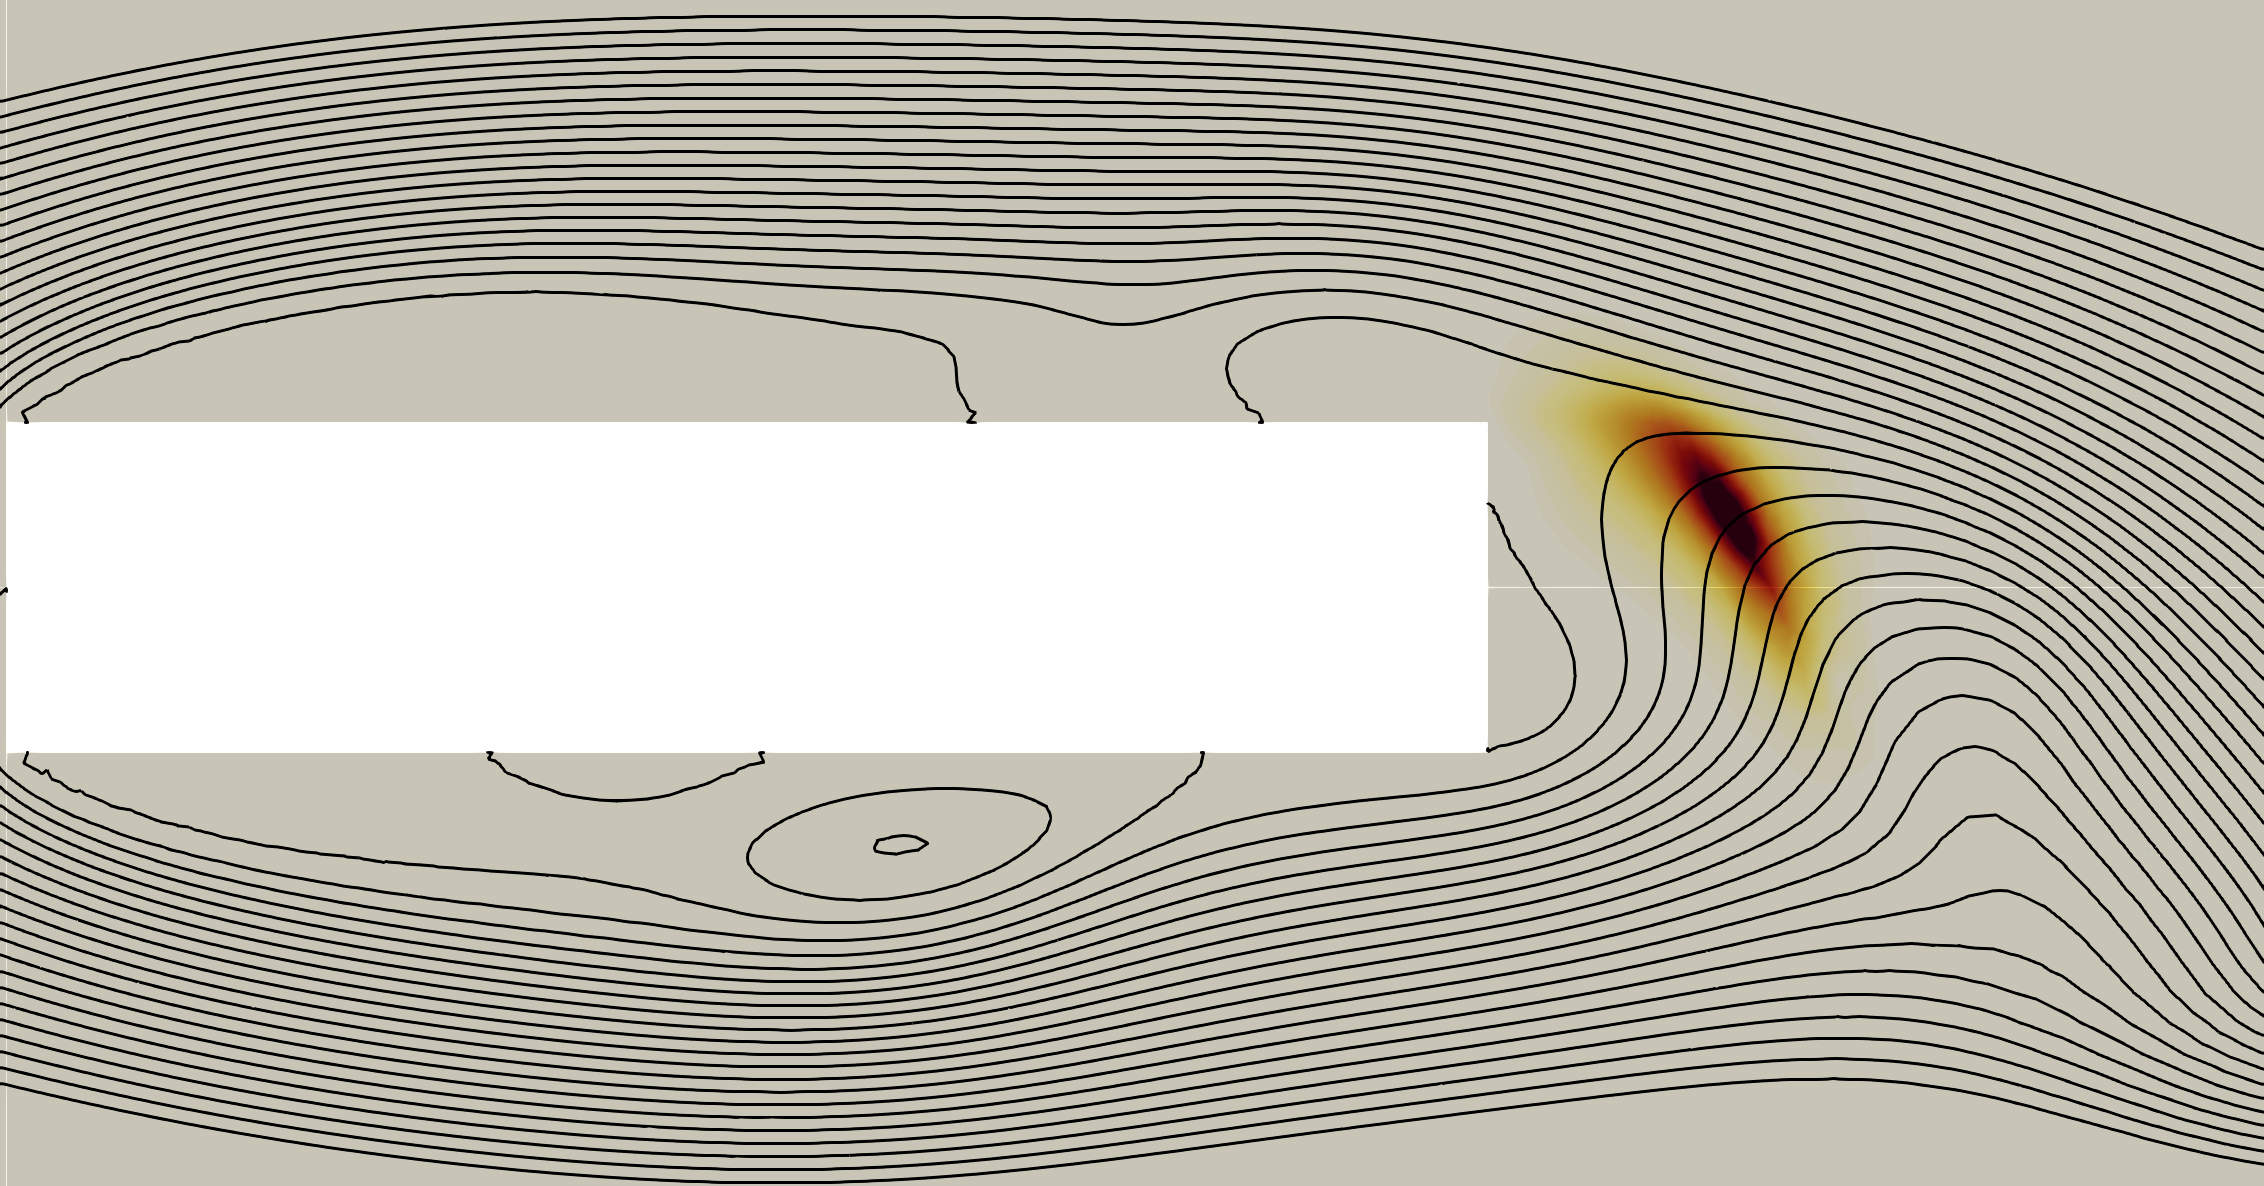
\includegraphics[width=0.49\textwidth]{./fig/AR4p5/sens3D_50.png}
  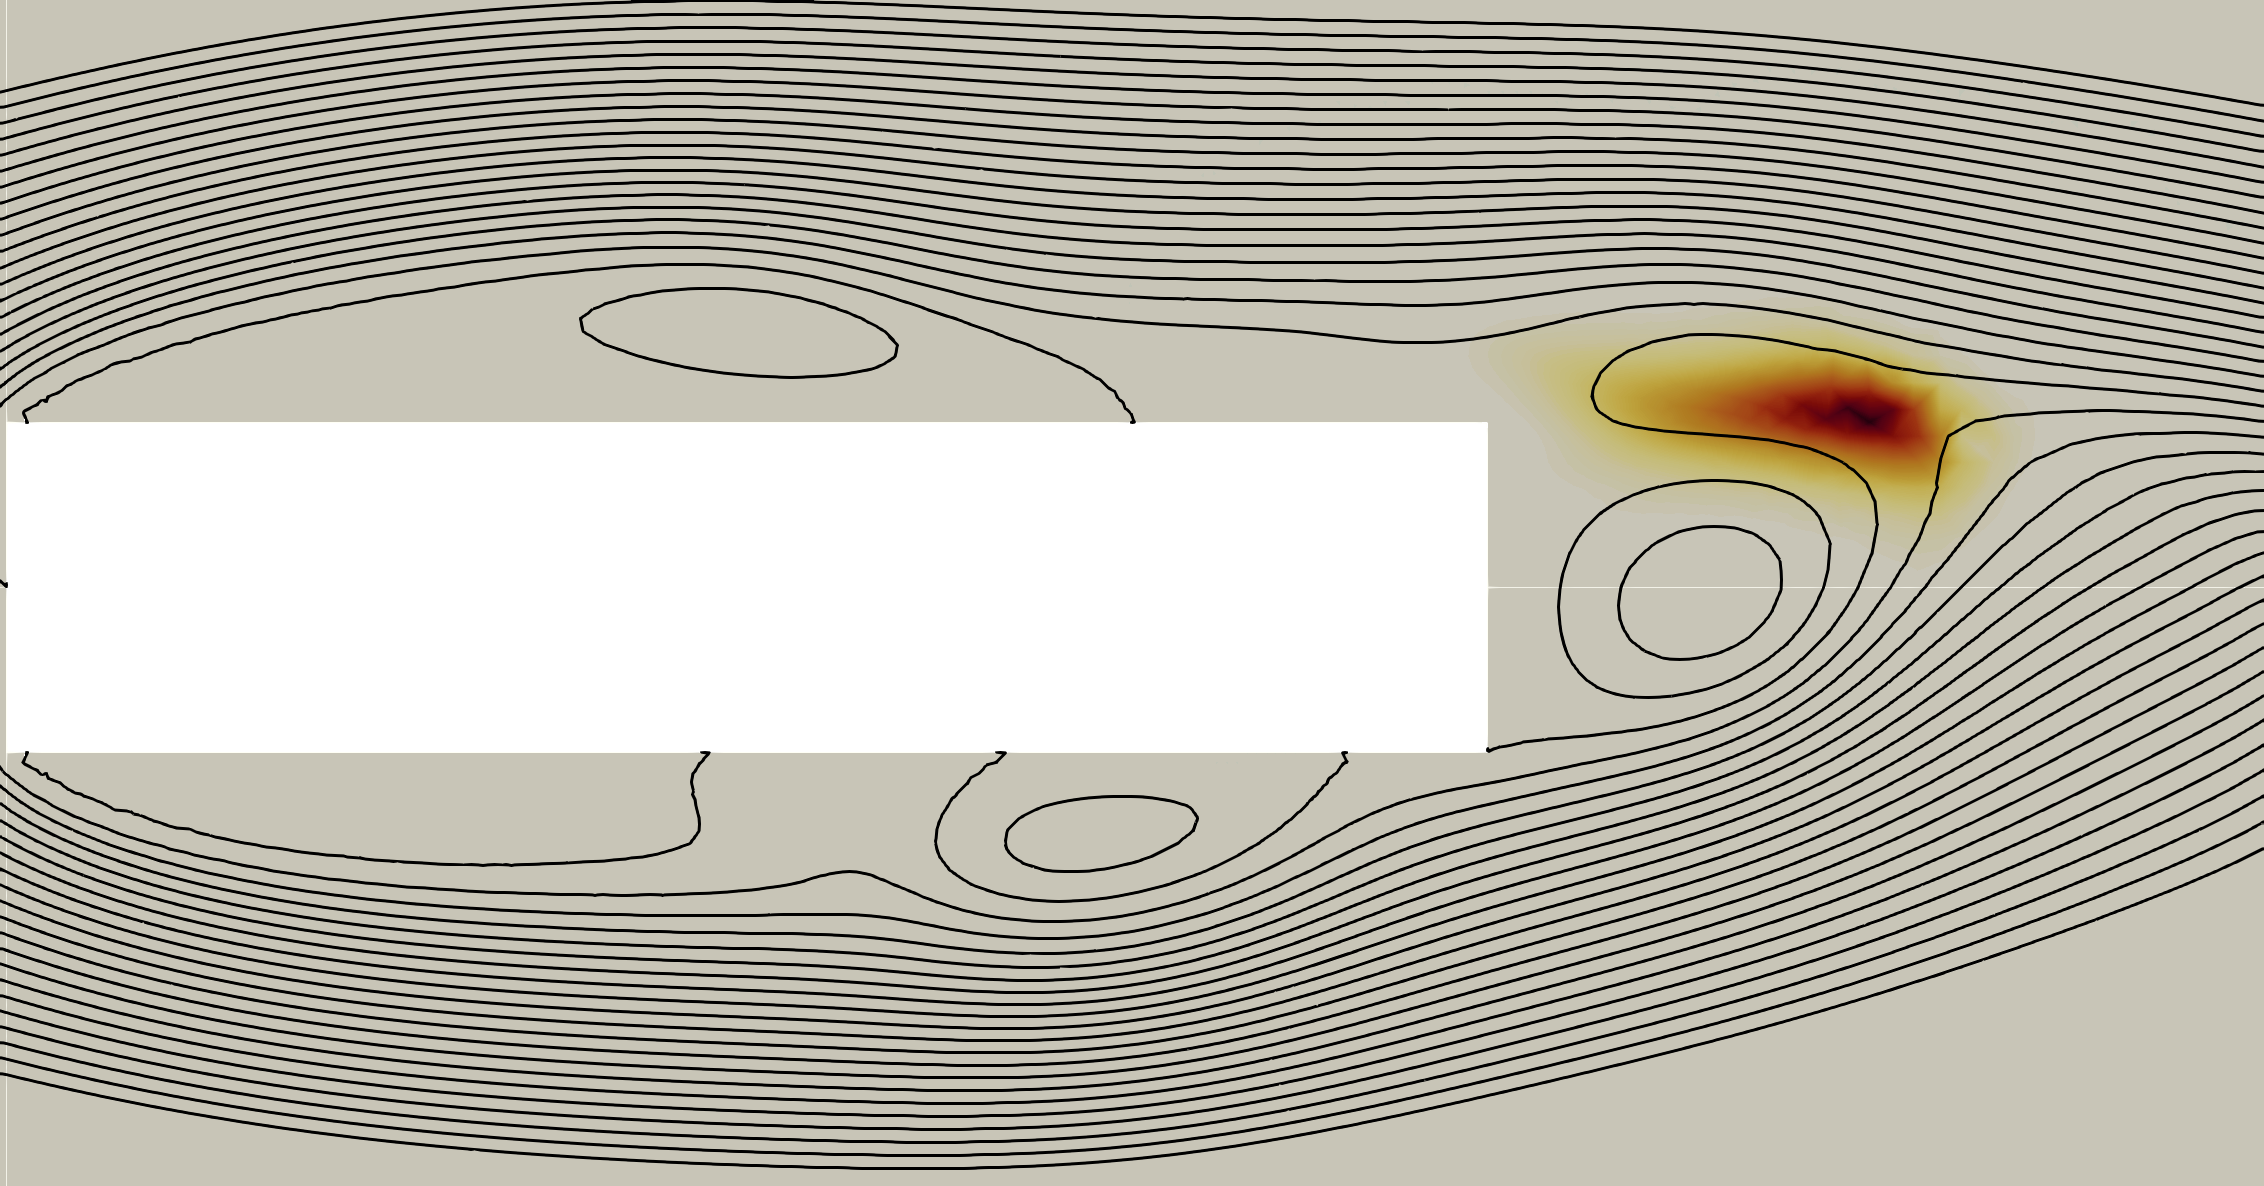
\includegraphics[width=0.49\textwidth]{./fig/AR4p5/sens3D_75.png}
  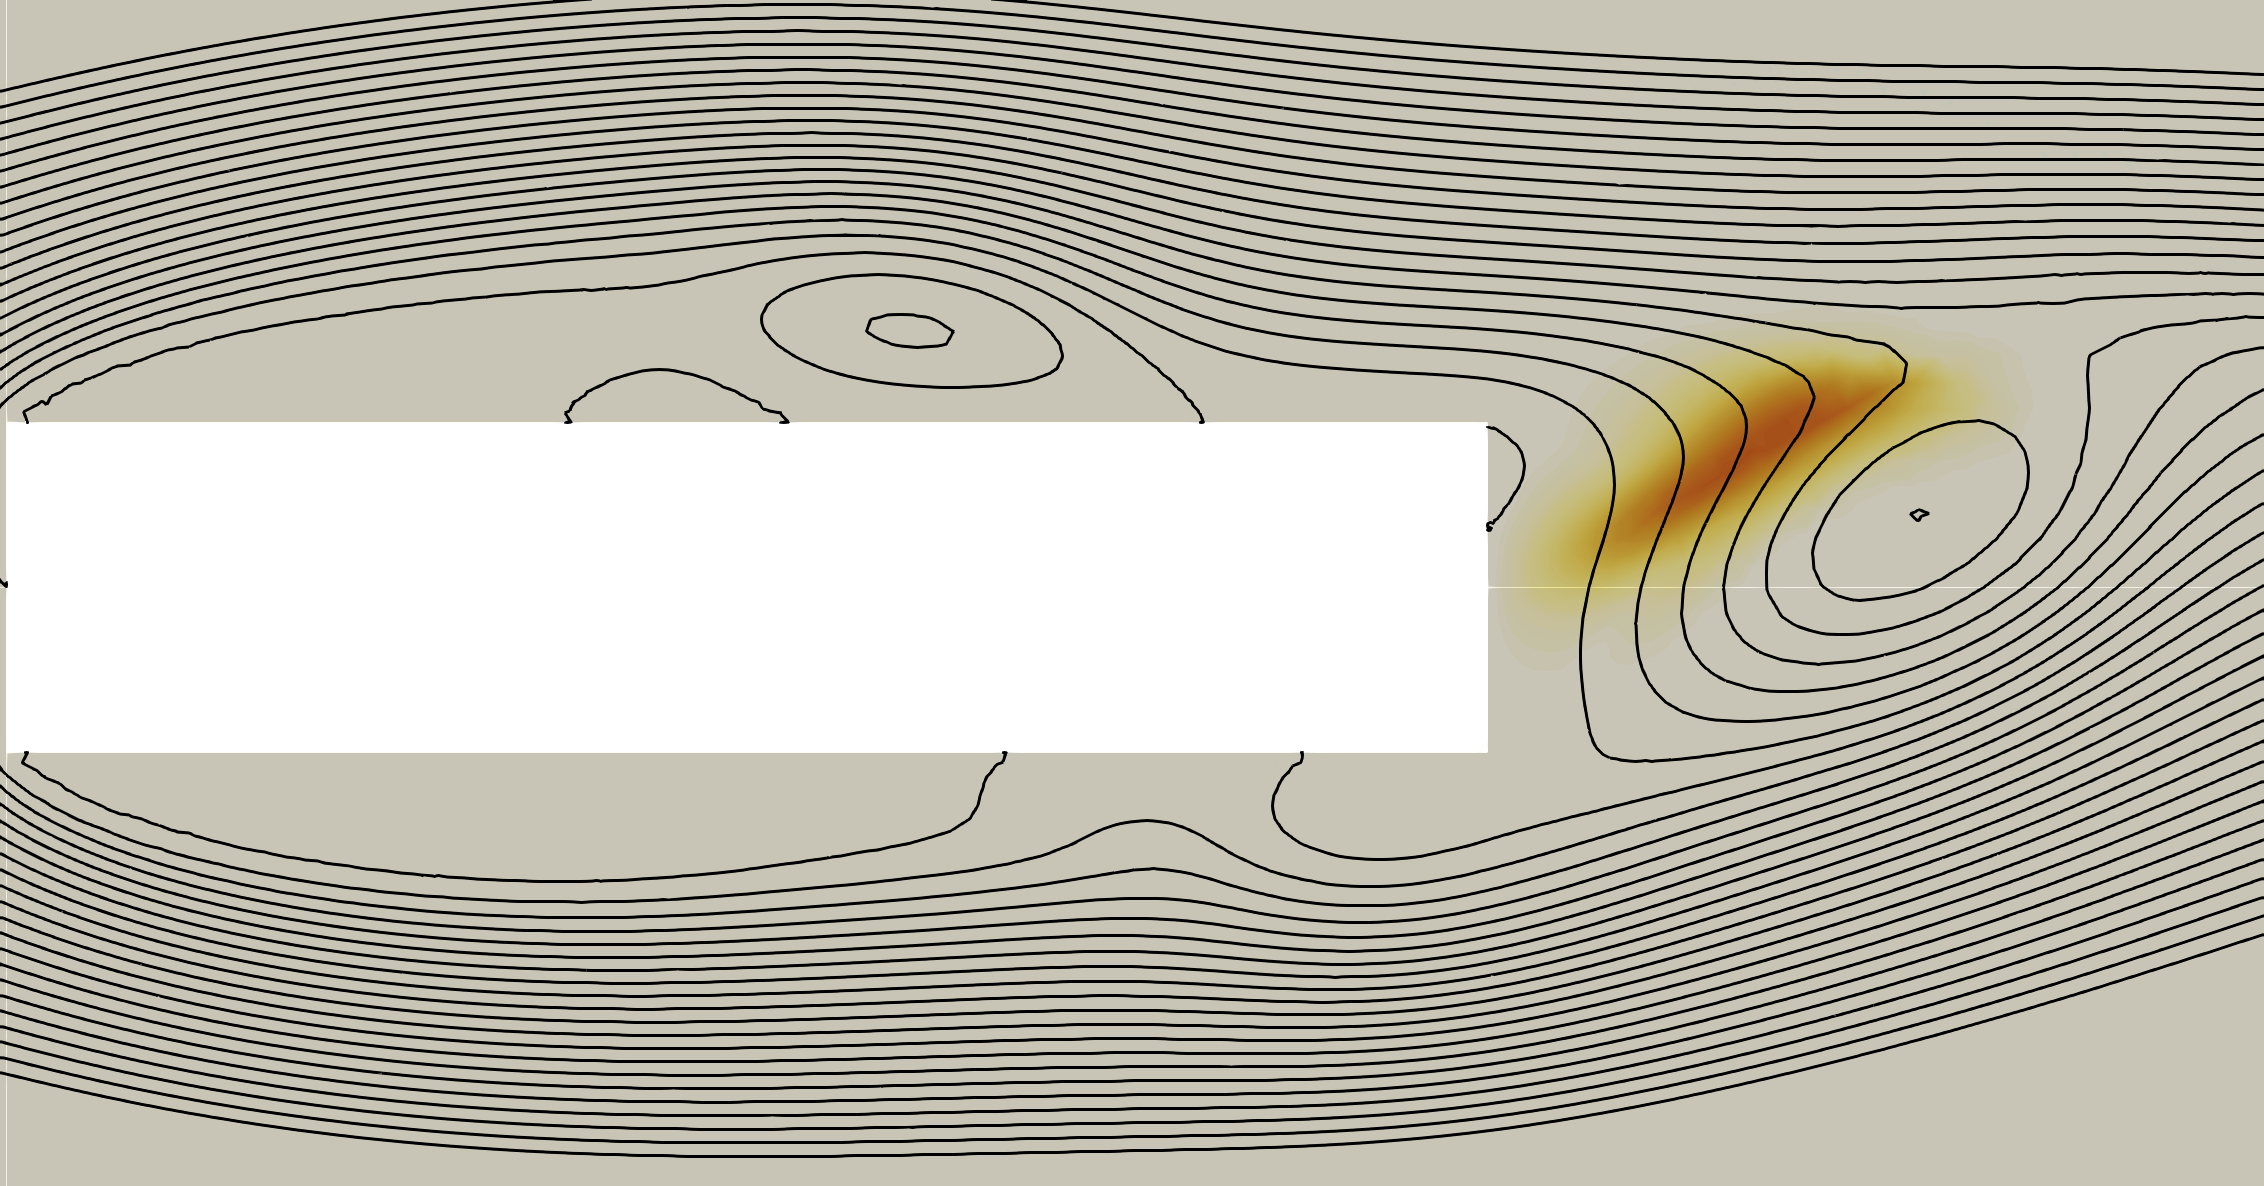
\includegraphics[width=0.49\textwidth]{./fig/AR4p5/sens3D_100.png}
  \caption{Structural sensitivity for $\AR=4.5$ and $\beta=8$ and $Re=450$ related to the 3D unstable mode. The four panels refer to four distinct time instants taken equispaced within the shedding period.}
  \label{fig:ss3d}
\end{figure}

\subsubsection{Non linear simulations}

\begin{figure}
  \centering
  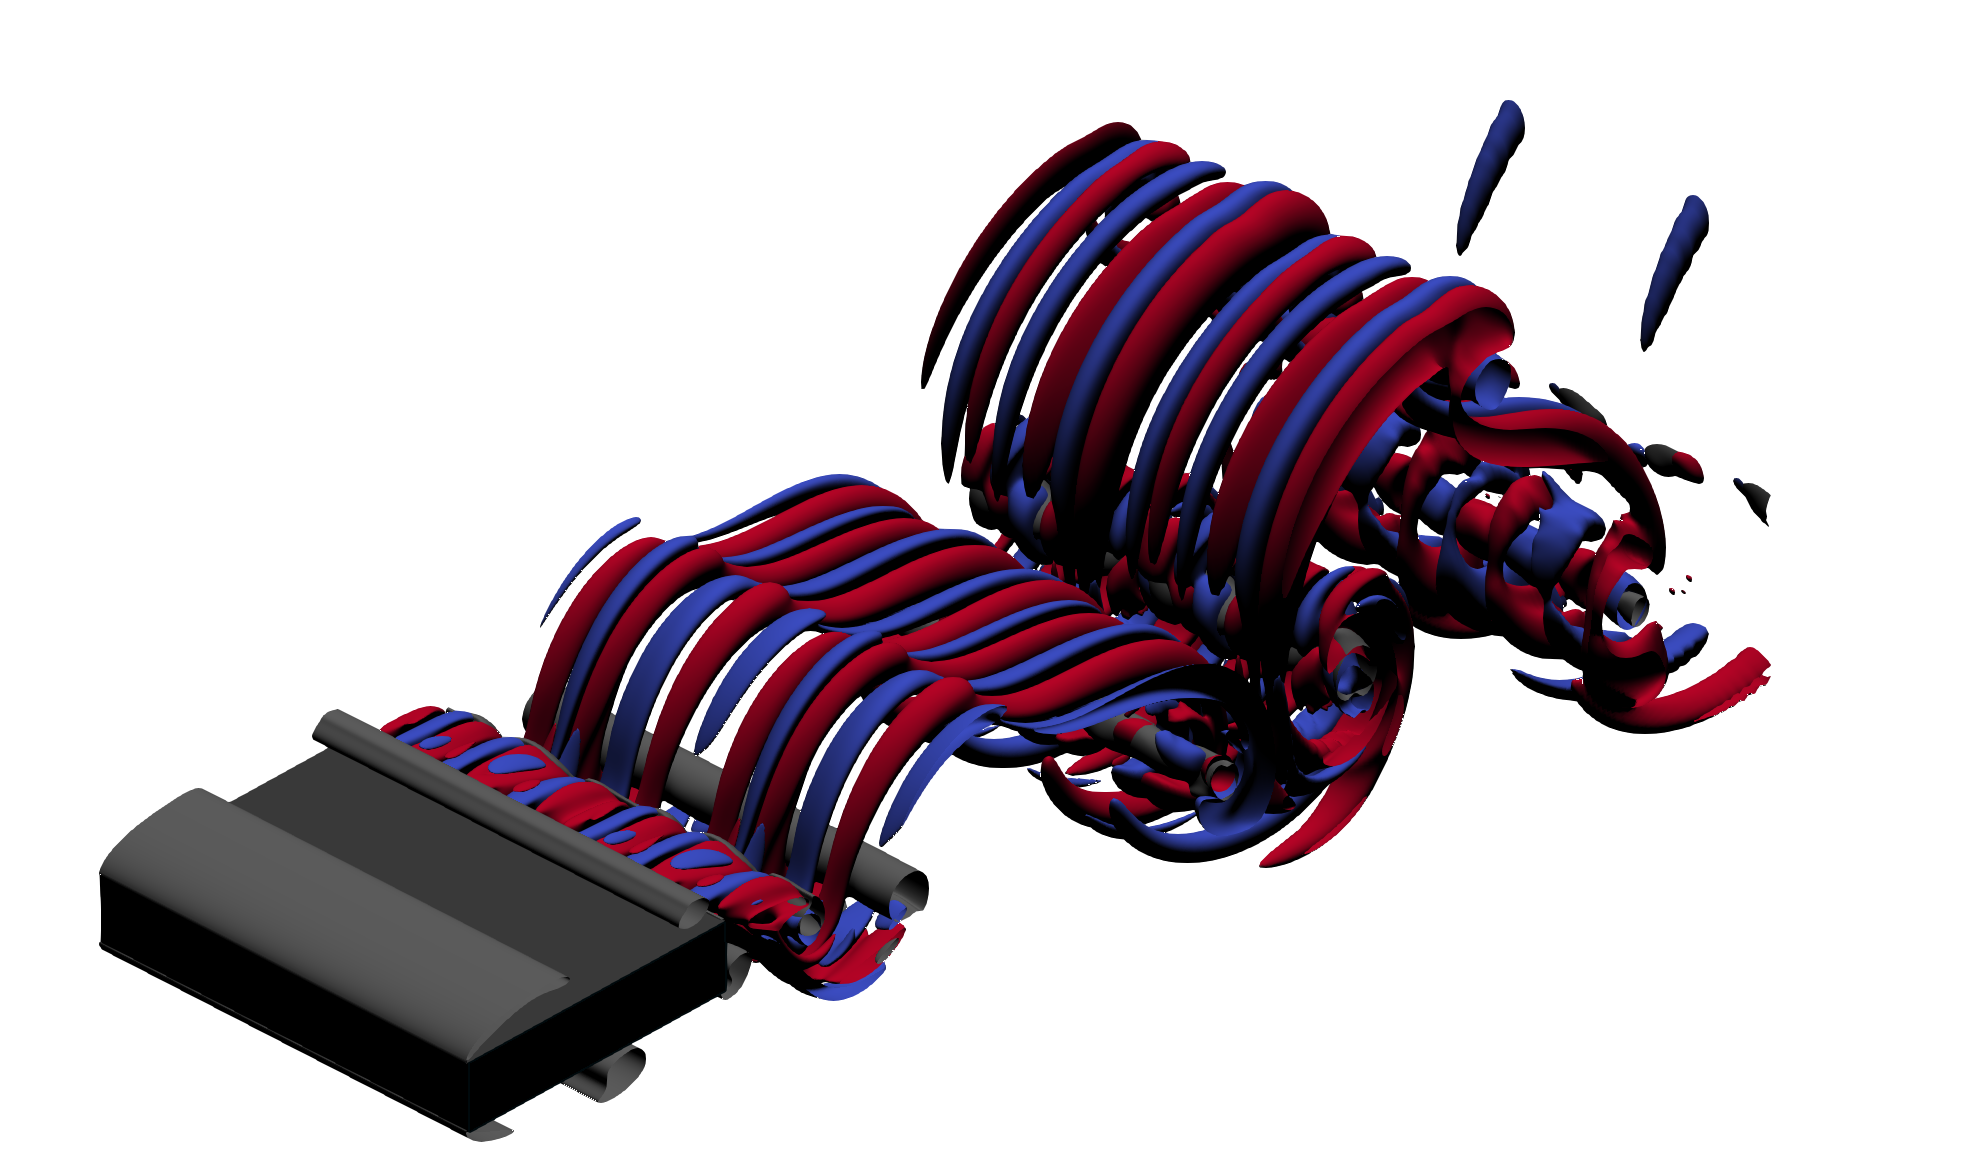
\includegraphics[width=0.7\textwidth]{./fig/AR4p5/lambda2_omegax-3D-Re450b.png}
  \caption{Results from the Direct numerical simulation at $\AR=4.5$ and $Re=450$. XX ADD THE SPECTRA OF THE FORCES XX}
  \label{fig:dns-ar4p5}
\end{figure}
%
A 3D DNS has been peroformed to confirm and expand the results of the Floquet analysis. They Reynolds number has been set to $Re=450$, i.e. above the critical value of $Re_{c3} \approx 420$ predicted by the Floquet analysis. The 2D potential flow solution has been used as initial condition. After the initial transient the simulation has been advanced for approximately \textcolor{red}{xx} shedding cycles with a variable times step to ensure a CFL numer below unity. The non linear simulation shows the the wake is defltected at these paramters and that the is three-dimensional. Specifically, by using iscontours of the instantaneous streamwise vorticity, figure \ref{} shows that the flow features a small-scale modulation in the spanwise direction with $\beta \approx 6$, which agrees with the most amplified wavenumber predicted by the Floquet analysis. The absence of any three-dimensionality along the lateral sides of the cylinder confirm that this is an unstable mode of the wake only. In terms of flow scales .. XX ADD XX
